\section{Упрощенный ДПТ}

\subsection{Инженерная форма ПФ}

Даны уравнения двигателя постоянного тока независимого возбуждения:
\begin{equation*}
    J\dot\omega=M,\ M=k_mI,\ I=\frac{U+\varepsilon_i}{R},\ \varepsilon_i=-k_e\omega. 
\end{equation*}
Найдем передаточную функцию для нашей системы(на вход $U(t)$, выход $\omega(t)$).
Подставив уравения друг в друга получаем дифференциальное уравнение (ДУ)
\begin{equation*}
    RJ\dot\omega+k_mk_e\omega=k_mU,
\end{equation*}
и далее передаточную функцию (ПФ)
\begin{equation*}
    W(s)=\frac{k_m}{RJs+k_mk_e},
\end{equation*}
откуда видно, что звено \textbf{реальное усилительное}:
\begin{equation*}
    W(s)=\frac{K}{Ts+1},
\end{equation*}
где $K=\frac{1}{k_e}$, $T=\frac{JR}{k_mk_e}$. Для моего варианта имею исходные данные
как в таблице \ref{tab:obj1}.
\begin{table}[H]
    \centering
    \begin{tabular}{|c|c|c|c|c|}
        \hline
        \( k_m,\ \text{Н$\cdot$м/А} \) & \( k_e,\ \text{В$\cdot$ с} \) & \( J,\ \text{кг$\cdot$ м$^2$} \) & \( R,\ \text{Ом} \) & \( L,\ \text{Гн} \) \\ 
        \hline
         0.3509  &  0.3509 &  0.0025  &  4.7320 & 1.0910 \\ 
        \hline
    \end{tabular}
    \label{tab:obj1}
    \caption{Данные по параметрам}
\end{table}
\noindent Тогда $\boldsymbol{K=2.8498}$, $\boldsymbol{T=0.0961}$.


\subsection{Весовая функция}

Весовую функцию ($\omega_{i.r.}(t)$) найдем из уравнения
\[
    \mathcal{L}\{\omega_{i.r.}(t)\} = W(s).
\]
Будем использовать инженерную форму:
\[
W(s)  = \frac{K}{T(s+\frac{1}{T})}= \frac{K}{T}\cdot\frac{1}{s+\frac{1}{T}},
\]
тогда, используя таблицу преобразований Лапсала, получаем
\[
\omega(t)= \frac{K}{T}e^{-\frac{t}{T}}.
\]
График этого решения и симуляцию можно посмотреть на рисунке \ref{fig:task_1_impl}.

\subsection{Переходная функция}

Выведем переходную функцию аналогично весовой из уравнения
\begin{equation*}
    s\cdot\mathcal L\{\omega_{s.r.}\}=W(s).
\end{equation*}
Рассмотрим
\[
\frac{W(s)}{s} = \frac{K}{T} \cdot \frac{1}{s\cdot(s + \frac{1}{T})}
=\frac{K}{T} \left( \frac{T}{s} - \frac{T}{s + \frac{1}{T}} \right).
\]
Используя таблицу преобразований Лапсала, получаем
\[
\omega_{s.r.}(t) = K \left( 1 - e^{-\frac{t}{T}} \right).
\]
График этого решения и симуляцию можно посмотреть на рисунке \ref{fig:task_1_step}.

\begin{figure}[htbp]
    \centering
    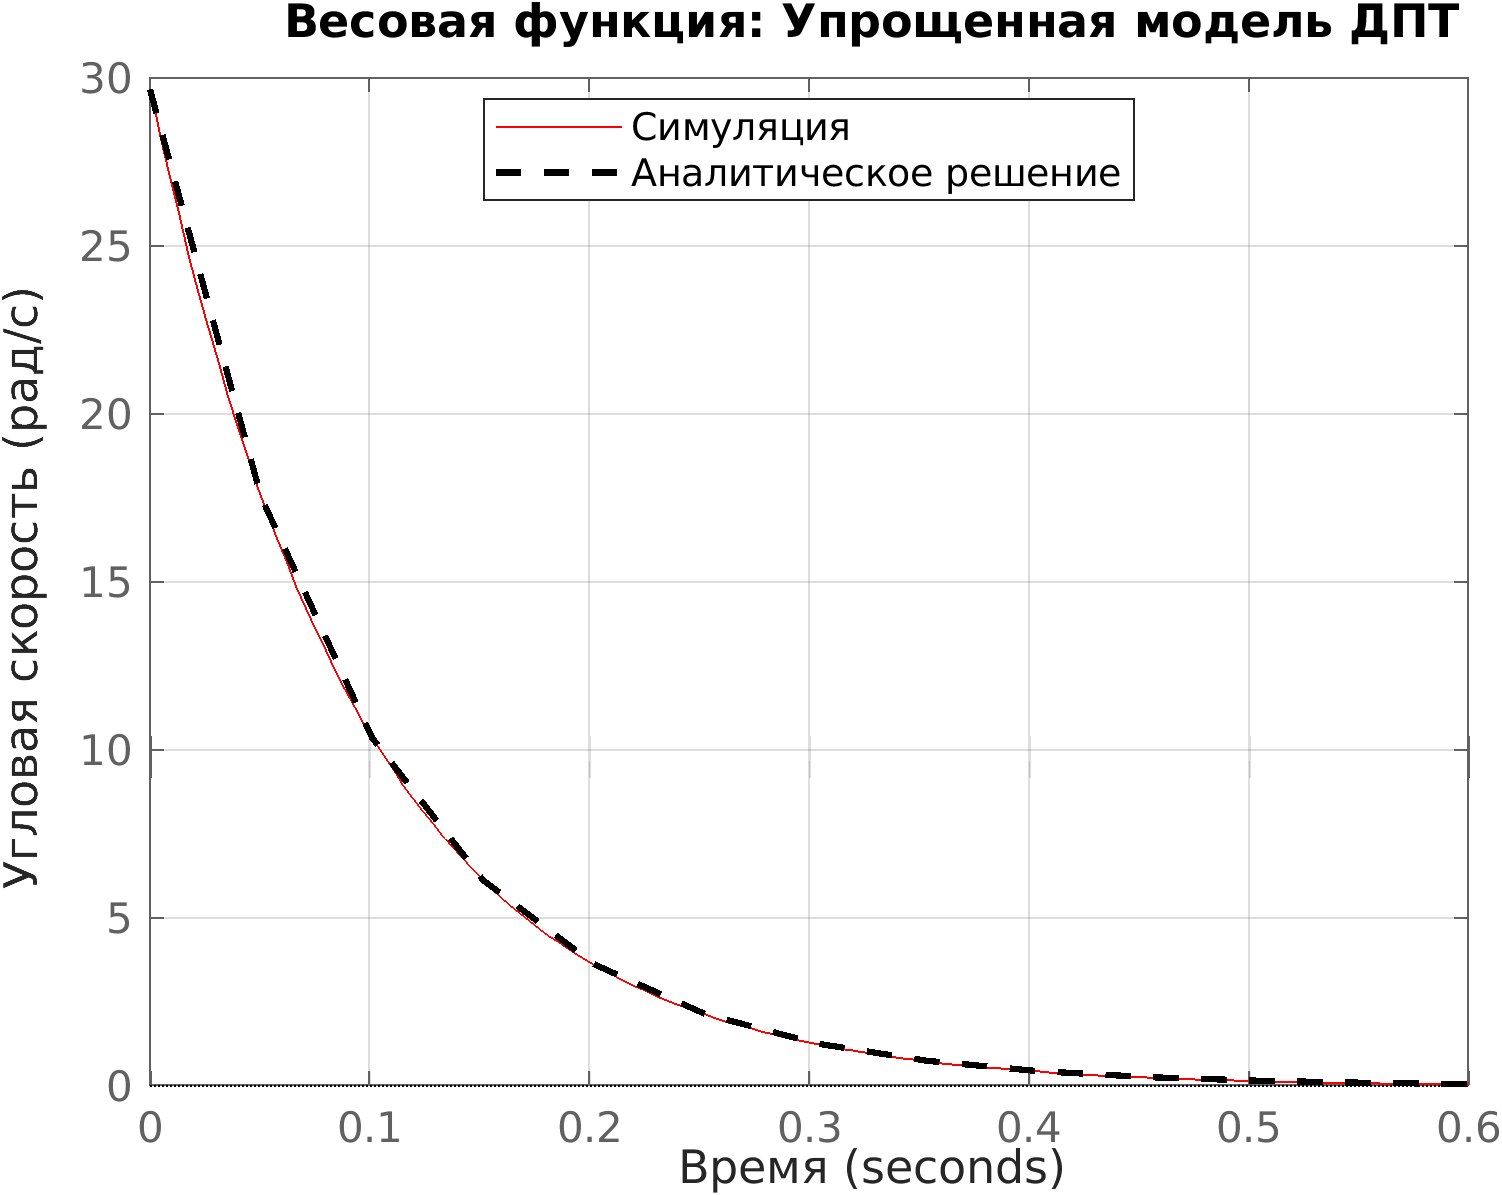
\includegraphics[width=0.7\textwidth]{figs/task_1_impl.png}
    \caption{Весовая функция упрощенной модели ДПТ.}
    \label{fig:task_1_impl}
\end{figure}

\begin{figure}[htbp]
    \centering
    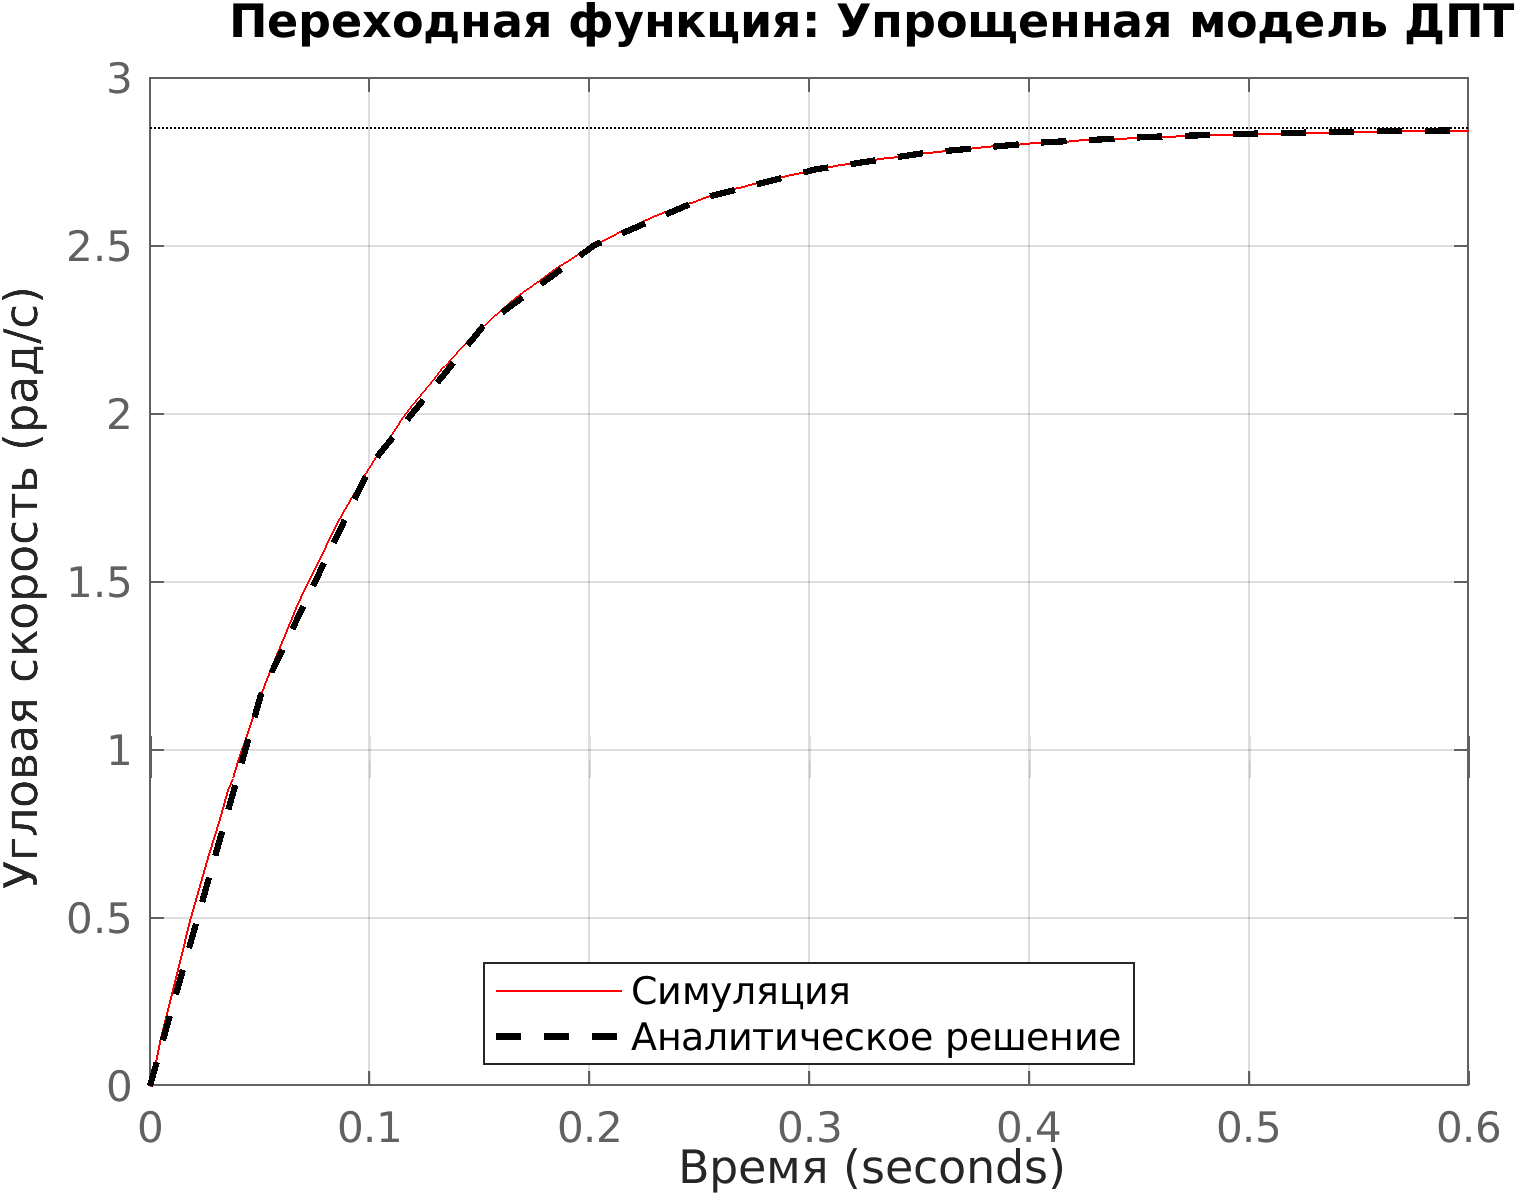
\includegraphics[width=0.7\textwidth]{figs/task_1_step.png}
    \caption{Переходная функция упрощенной модели ДПТ.}
    \label{fig:task_1_step}
\end{figure}

\subsection{Частотные характеристики}

Получим формулы для АЧХ, ФЧХ и ЛАФЧХ.
\begin{equation*}
    W(j\omega)=\frac{K}{Tj\omega + 1}=\frac{K(1-Tj\omega)}{1+\omega^2T^2}
    =\frac{K}{1+\omega^2T^2}+j\frac{-\omega TK}{1+\omega^2T^2},
\end{equation*}
обозначим вещественную и мнимую части:
\begin{equation*}
    U(\omega)=\frac{K}{1+\omega^2T^2},\quad V(\omega)=-\frac{\omega TK}{1+\omega^2T^2}.
\end{equation*}
Теперь можем вычислить амплитуду, фазу и :
\begin{equation*}
    A(\omega)=\sqrt{U(\omega)^2+V(\omega)^2},\quad \varphi(\omega)=\text{atan2}\left( V(\omega), U(\omega) \right),
    \quad L(\omega)=20\log_{10}\frac{A(\omega)}{A_\text{б}}.
\end{equation*}
Амплитуду можем вычислить конкретнее:
\begin{equation*}
    A(\omega)
    =\sqrt{\frac{K^2}{(1+\omega^2T^2)^2}+\frac{(\omega TK)^2}{(1+\omega^2T^2)^2}}
    =\frac{K\sqrt{1+\omega^2T^2}}{1+\omega^2T^2}
    =\frac{K}{\sqrt{1+\omega^2T^2}}.
\end{equation*}
Графики АФЧХ и ЛАФЧХ можно посмотреть на рисунке \ref{fig:task_1_АФЧХ} и \ref{fig:task_1_ЛАФЧХ}.

\begin{figure}[H]
    \centering
    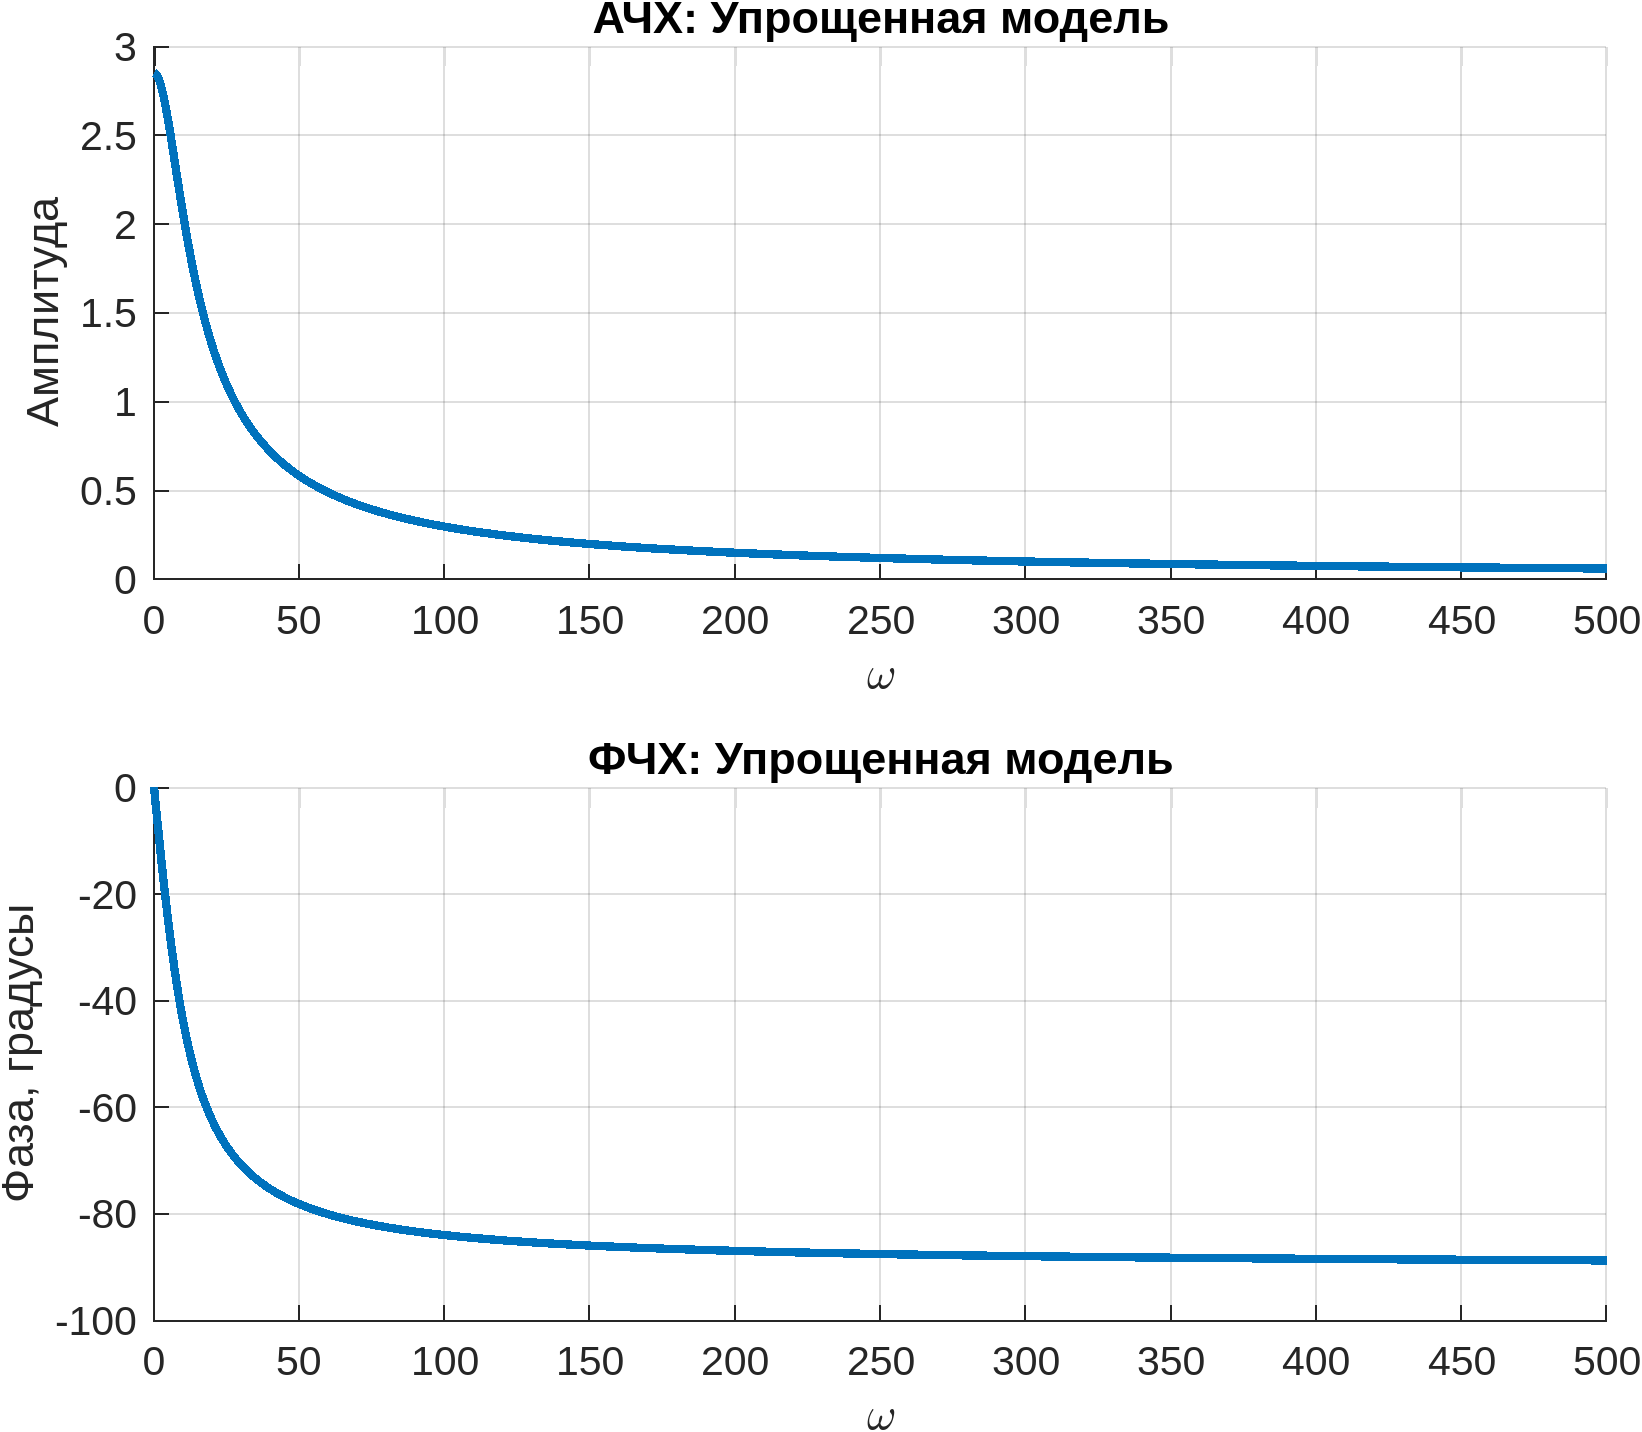
\includegraphics[width=0.7\textwidth]{figs/task_1_АФЧХ.png}
    \caption{АФЧХ упрощенной модели ДПТ.}
    \label{fig:task_1_АФЧХ}
\end{figure}

\begin{figure}[H]
    \centering
    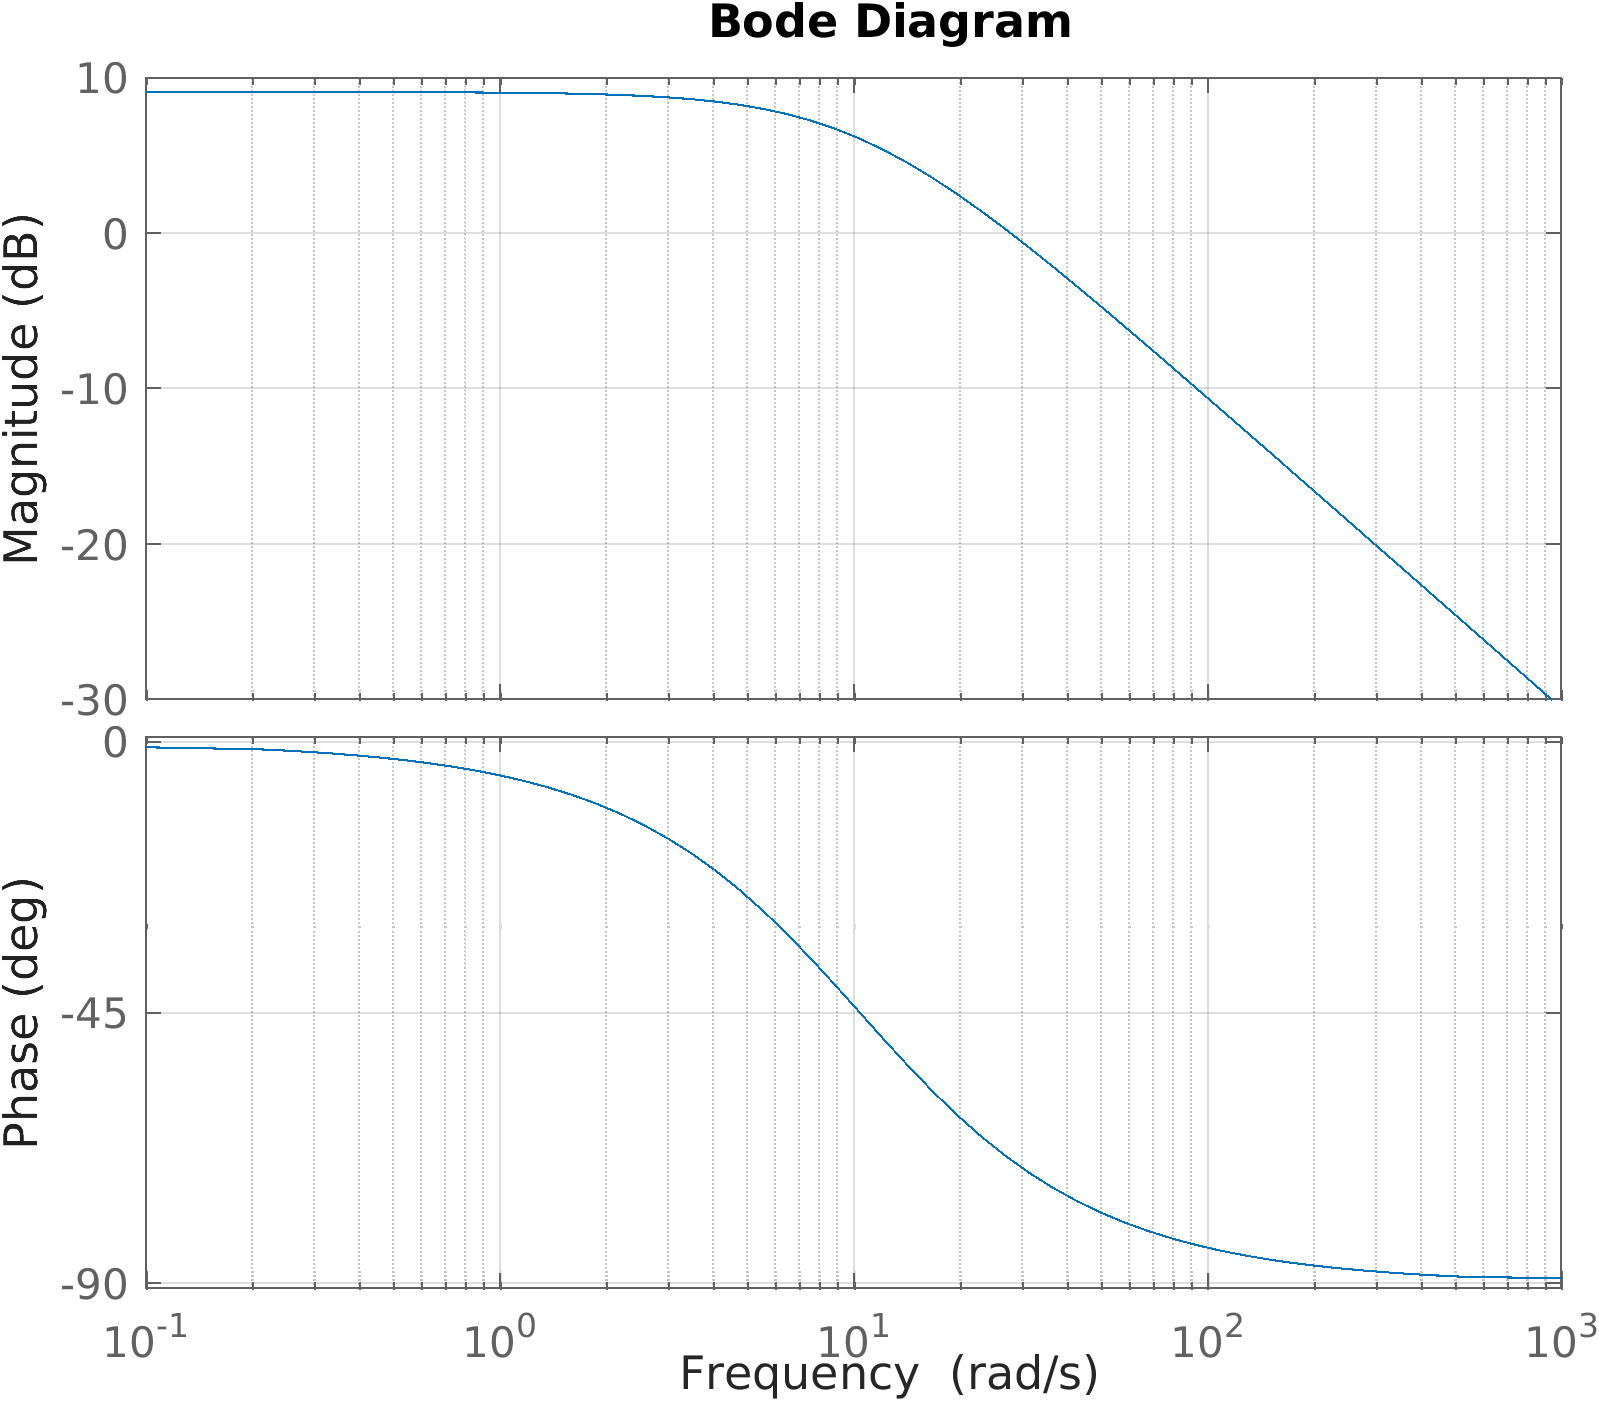
\includegraphics[width=0.7\textwidth]{figs/task_1_ЛАФЧХ.png}
    \caption{ЛАФЧХ упрощенной модели ДПТ.}
    \label{fig:task_1_ЛАФЧХ}
\end{figure}


\section{Полный ДПТ}

\subsection{Инженерная форма ПФ}

Даны уравнения двигателя постоянного тока независимого возбуждения:
\begin{equation*}
    J\dot\omega=M,\ M=k_mI,\ I=\frac{U+\varepsilon}{R},\ \varepsilon=\varepsilon_i+\varepsilon_s,\ 
    \varepsilon_i=-k_e\omega,\ \varepsilon_s=-L\dot I. 
\end{equation*}
Найдем передаточную функцию для нашей системы(на вход $U(t)$, выход $\omega(t)$).
Подставив уравения друг в друга получаем дифференциальное уравнение (ДУ)
\[
JL\ddot{\omega} + JR\dot{\omega} + k_{m}k_{e}\omega = k_mU,
\]
и далее передаточную функцию (ПФ)
\[
W(s) = \frac{k_m}{JLs^2 + JRs +  k_m k_e}.
\]
Она может быть либо апериодическим звеном 2го порядка, либо колебательным,
найдем дискриминант знаменателя, используя данные из таблицы \ref{tab:obj1}, 
чтобы решить какой тип звена.
\begin{equation*}
    D=J^2R^2-4JLk_{m}k_{e}=-0.0012,\ \text{то есть \textbf{звено колебательное}}.
\end{equation*}
Инженерный вид колебательного звена
\begin{equation*}
    W(s)=\frac{K}{T^2s^2+2\xi T s+1},
\end{equation*}
где в нашем случае $K=\frac{1}{k_{e}}=2.8498$, $T=\sqrt \frac{JL}{k_{m}k_{e}}=0.1490$, 
$\xi=\frac{R\sqrt{J}}{2\sqrt{Lk_mk_e}}=0.3228$.

\subsection{Весовая функция}

Выведем весовую функцию, которая является ПФ во временной области. Для начала
нужно получить полный квадрат в знаменателе:
\begin{equation*}
    W(s)=\frac{K}{(Ts+\xi)^2-\xi^2+1}
    =\frac{\frac{K}{T^2}}{\left(s+\frac{\xi}{T}\right)^2+\frac{1}{T^2}(1-\xi^2)},
\end{equation*}
видно, что ПФ похожа на экспоненту с синусом
\begin{equation*}
    \mathcal L \{e^{\alpha t}\sin(\omega t)\}=\frac{\omega}{(s-\alpha)^2+\omega^2},
\end{equation*}
где $\omega=\frac{1}{T}\sqrt{1-\xi^2}$, $\alpha=-\frac{\xi}{T}$. Пусть $\frac{K}{T^2}=\beta\omega$,
тогда $\beta=\frac{K}{T\sqrt{1-\xi^2}}$. Запишем весовую функцию
\begin{equation*}
    \omega_{i.r.}=\frac{K}{T\sqrt{1-\xi^2}}\exp{\left(-\frac{\xi}{T}t\right)}\sin\left(\frac{t}{T}\sqrt{1-\xi^2}\right).
\end{equation*}
Ее график и симуляцию можно посмотреть на рисунке \ref{fig:task_2_impl}, все сходится.

\begin{figure}[htbp]
    \centering
    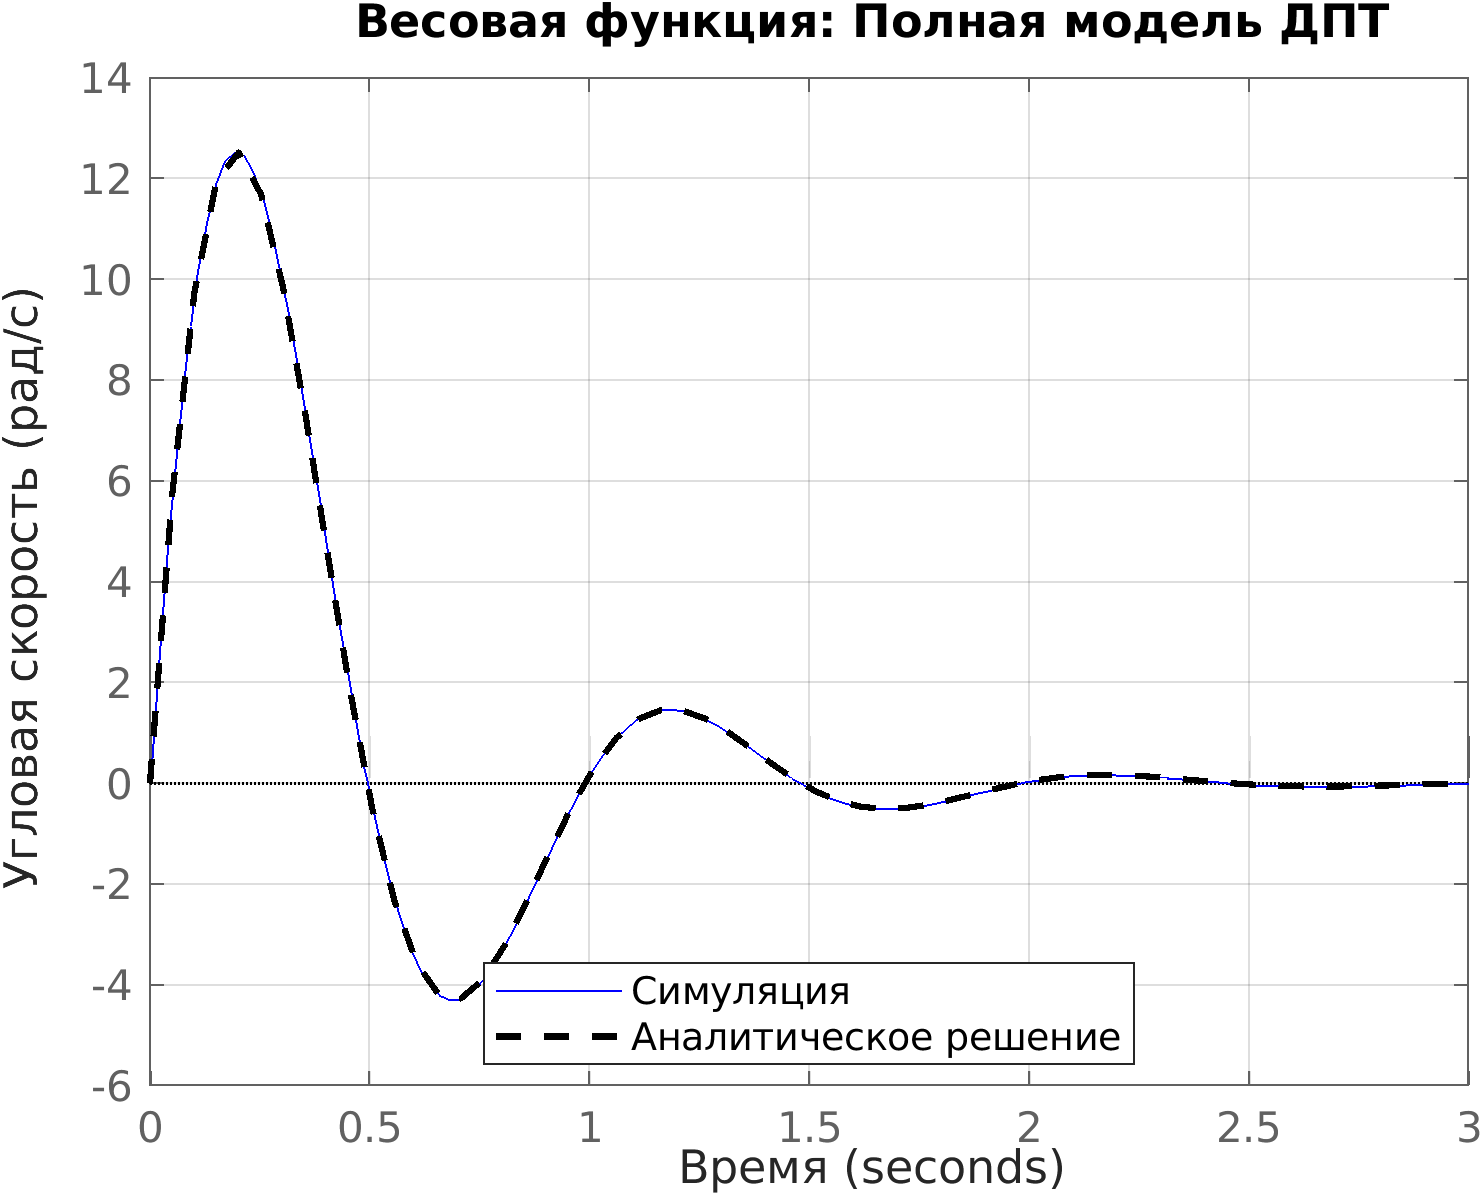
\includegraphics[width=0.7\textwidth]{figs/task_2_impl.png}
    \caption{Весовая функция полной модели ДПТ.}
    \label{fig:task_2_impl}
\end{figure}

\subsection{Переходная функция}

Выведем переходную функцию аналогично весовой из уравнения
\begin{equation*}
    s\cdot\mathcal L\{\omega_{s.r.}\}=W(s).
\end{equation*}
Для начала приется разложить на простые дроби
\begin{equation*}
    \frac{W(s)}{s}=\frac{K}{s((Ts+\xi)^2-\xi^2+1)}=\frac{A}{s}+\frac{Bs+C}{(Ts+\xi)^2-\xi^2+1},
\end{equation*}
что делается через решение СЛАУ
\begin{equation*}
    \begin{cases}
        K=A,\\
        0=C+2AT\xi,\\
        0=AT^2+B,
    \end{cases}\Rightarrow
    \begin{cases}
        A=K,\\
        C=-2KT\xi,\\
        B=-KT^2.
    \end{cases}
\end{equation*}
Получаем
\begin{equation*}
    \frac{W(s)}{s}=\frac{K}{s}+\frac{-KT^2s-2KT\xi}{(Ts+\xi)^2-\xi^2+1}.
\end{equation*}
Рассмотрим второе слагаемое отдельно, используя разложение знаменателя из
предыдущего пункта
\begin{multline*}
    \frac{-KT^2s-2KT\xi}{(Ts+\xi)^2-\xi^2+1}
    =\frac{-K(s+\frac{2\xi}{T})}{\left(s+\frac{\xi}{T}\right)^2+\frac{1}{T^2}(1-\xi^2)}
    =-K\left[
        \frac{s+\frac{\xi}{T}}{\left(s+\frac{\xi}{T}\right)^2+\frac{1}{T^2}(1-\xi^2)}
        +\frac{\frac{\xi}{T}}{\left(s+\frac{\xi}{T}\right)^2+\frac{1}{T^2}(1-\xi^2)}
    \right].
\end{multline*}
Пусть $\frac{\xi}{T}=\beta\omega$, тогда $\beta=\frac{\xi}{\sqrt{1-\xi^2}}$. Теперь сможем
получить переходную функцию с помощью табличных образов Лапласа
\begin{equation*}
    \omega_{s.r.}=K-K\cdot\exp{\left(-\frac{\xi}{T}t\right)}\cdot\left[\cos\left(\frac{t}{T}\sqrt{1-\xi^2}\right)+\frac{\xi}{\sqrt{1-\xi^2}}\sin\left(\frac{t}{T}\sqrt{1-\xi^2}\right)\right].
\end{equation*}
Ее график и симуляцию можно посмотреть на рисунке \ref{fig:task_2_step}, все сходится.

\begin{figure}[htbp]
    \centering
    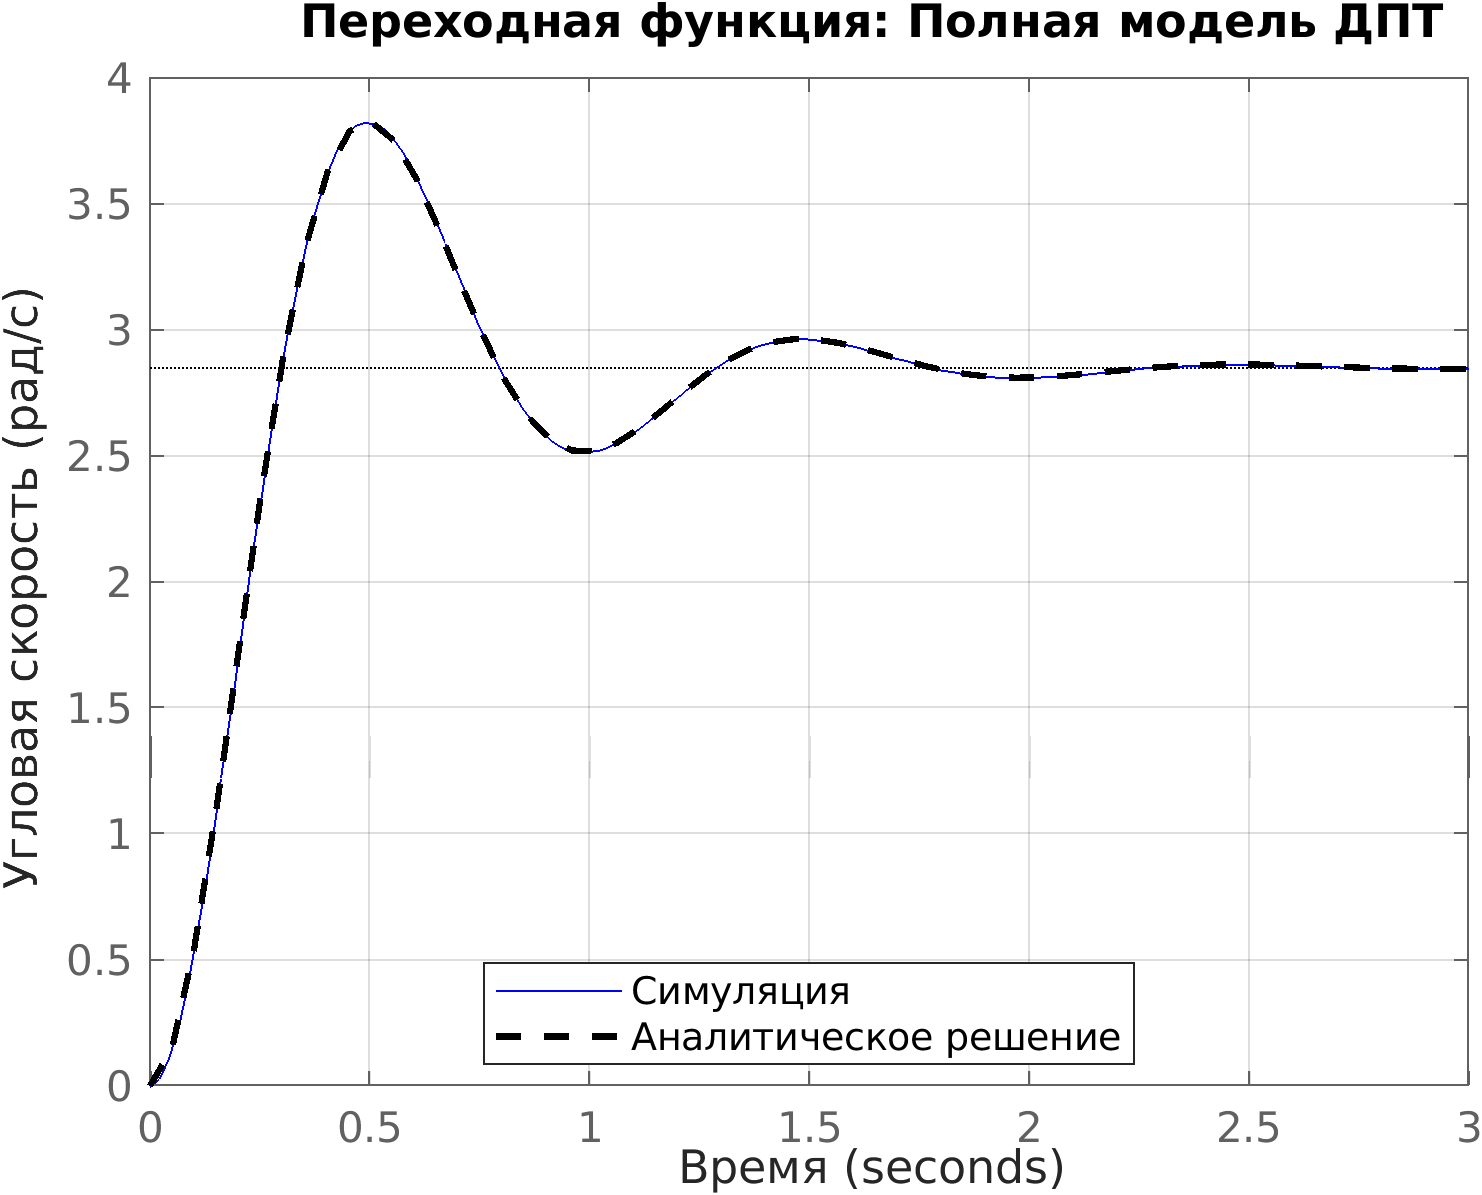
\includegraphics[width=0.7\textwidth]{figs/task_2_step.png}
    \caption{Переходная функция полной модели ДПТ.}
    \label{fig:task_2_step}
\end{figure}


\subsection{Частотные характеристики}

Получим формулы для АЧХ и ФЧХ.
\begin{equation*}
    \begin{split}
        &W(j\omega)=\frac{K}{T^2(j\omega)^2+2\xi T (j\omega)+1},\\
        &D=4\xi^2T^2-4T^2=4T^2(\xi^2-1)\approx-0.080,\\
        &i\omega=\frac{-2\xi T\pm\sqrt{D}}{2T^2}\approx-2.166\pm j6.352,\\
        &W(j\omega)=\frac{K}{(2.166+j(\omega-6.352))(2.166+j(\omega+6.352))}=\frac{K}{A_1(\omega)A_2(\omega)}e^{-j(\varphi_1(\omega)+\varphi_2(\omega))},
    \end{split}
\end{equation*}
где 
\begin{equation*}
    \begin{aligned}
        A_1(\omega)=\sqrt{2.166^2+(\omega-6.352)^2},&\quad \varphi_1(\omega)=\arctg\left(\frac{\omega-6.352}{2.166}\right),\\
        A_2(\omega)=\sqrt{2.166^2+(\omega+6.352)^2},&\quad \varphi_2(\omega)=\arctg\left(\frac{\omega+6.352}{2.166}\right).
    \end{aligned}
\end{equation*}
Тогда амплитуда, фаза и ЛАЧХ вычисляются так
\begin{equation*}
    A(\omega)=\frac{K}{A_1(\omega)A_2(\omega)},\quad \varphi(\omega)=-\varphi_1(\omega)-\varphi_2(\omega),\quad L(\omega)=20(\log_{10}K-\log_{10}A_1(\omega)-\log_{10}A_2(\omega)).
\end{equation*}
Графики АФЧХ и ЛАФЧХ можно посмотреть на рисунках \ref{fig:task_2_АФЧХ} и \ref{fig:task_2_ЛАФЧХ}.

\begin{figure}[H]
    \centering
    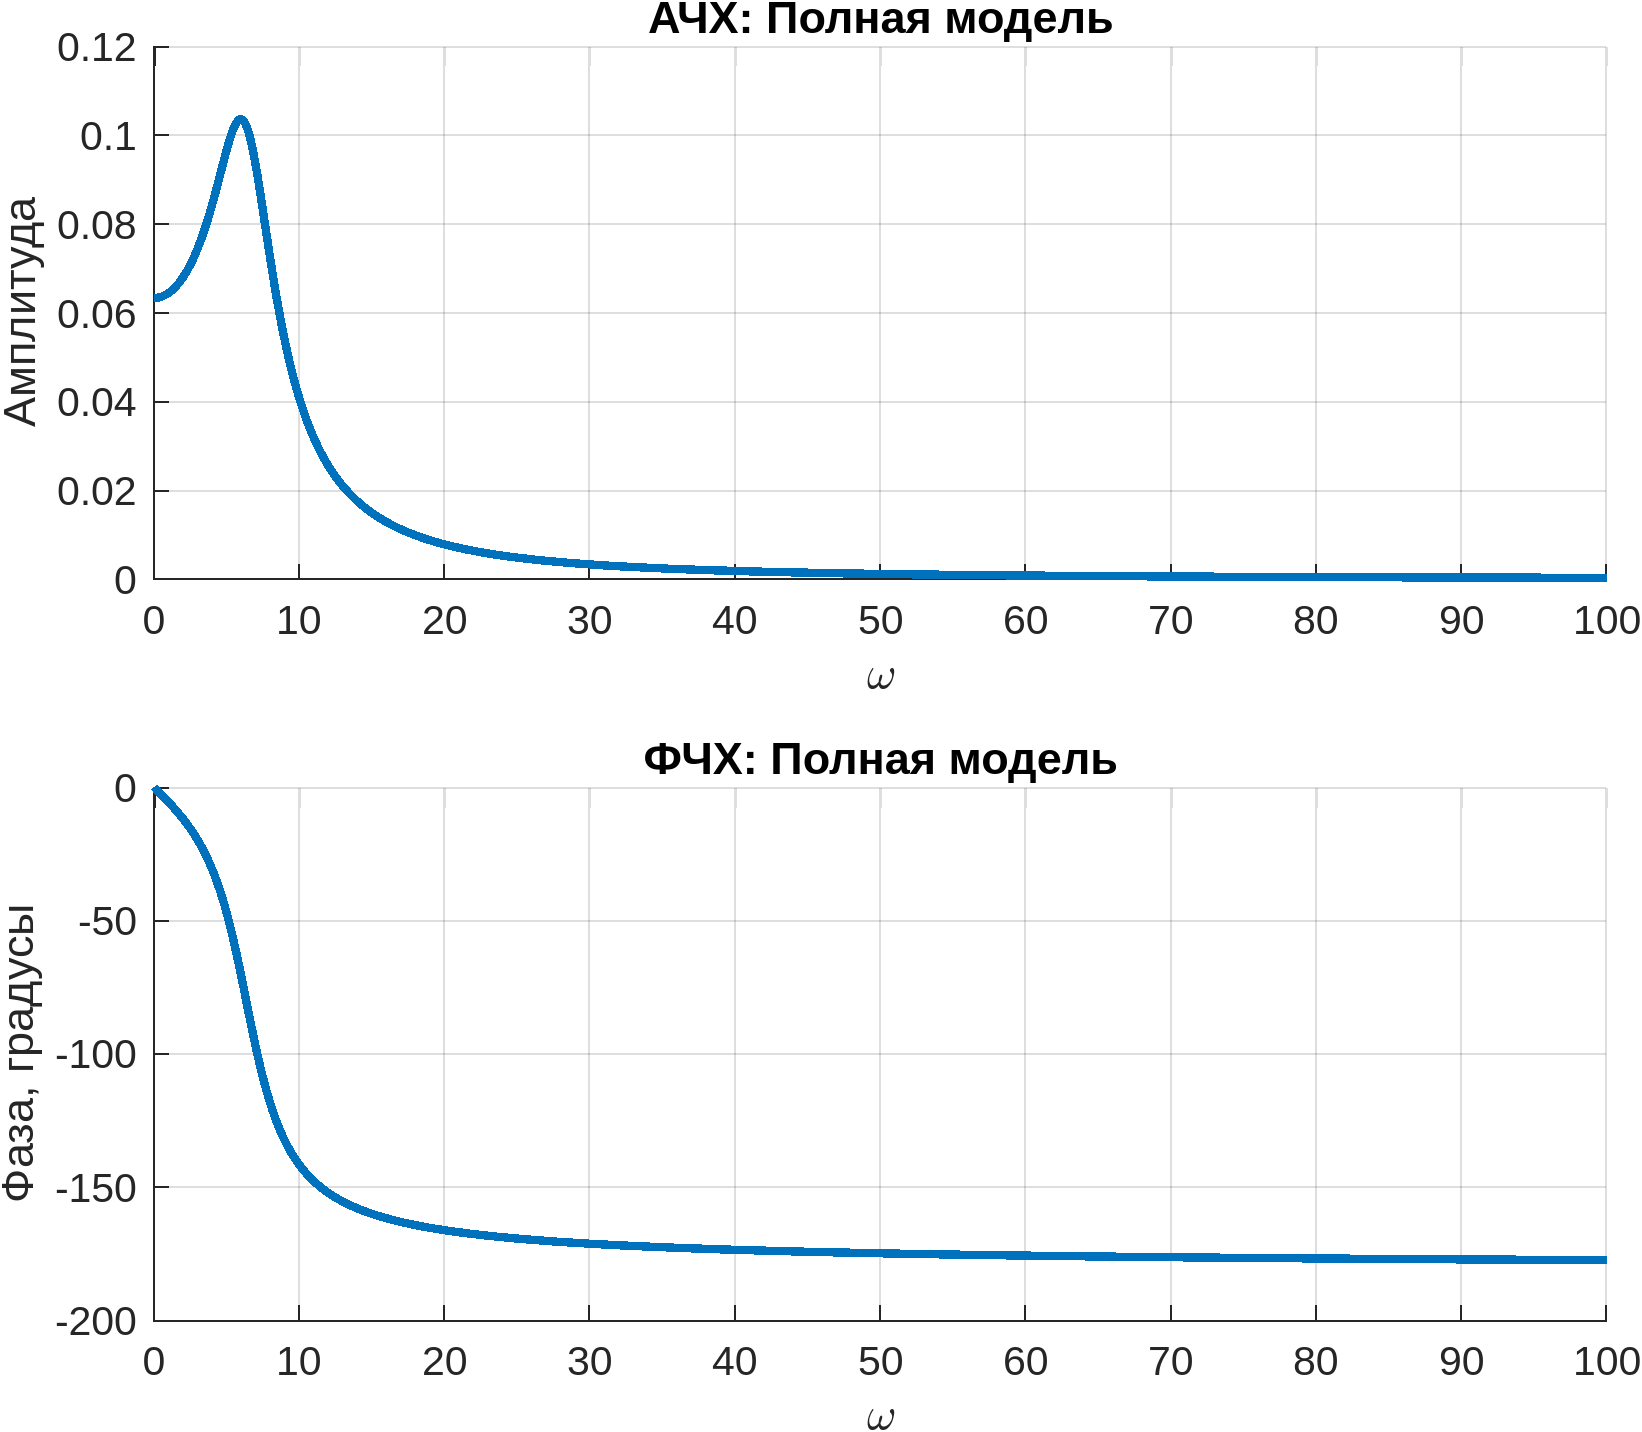
\includegraphics[width=0.7\textwidth]{figs/task_2_АФЧХ.png}
    \caption{АФЧХ полной модели ДПТ.}
    \label{fig:task_2_АФЧХ}
\end{figure}

\begin{figure}[H]
    \centering
    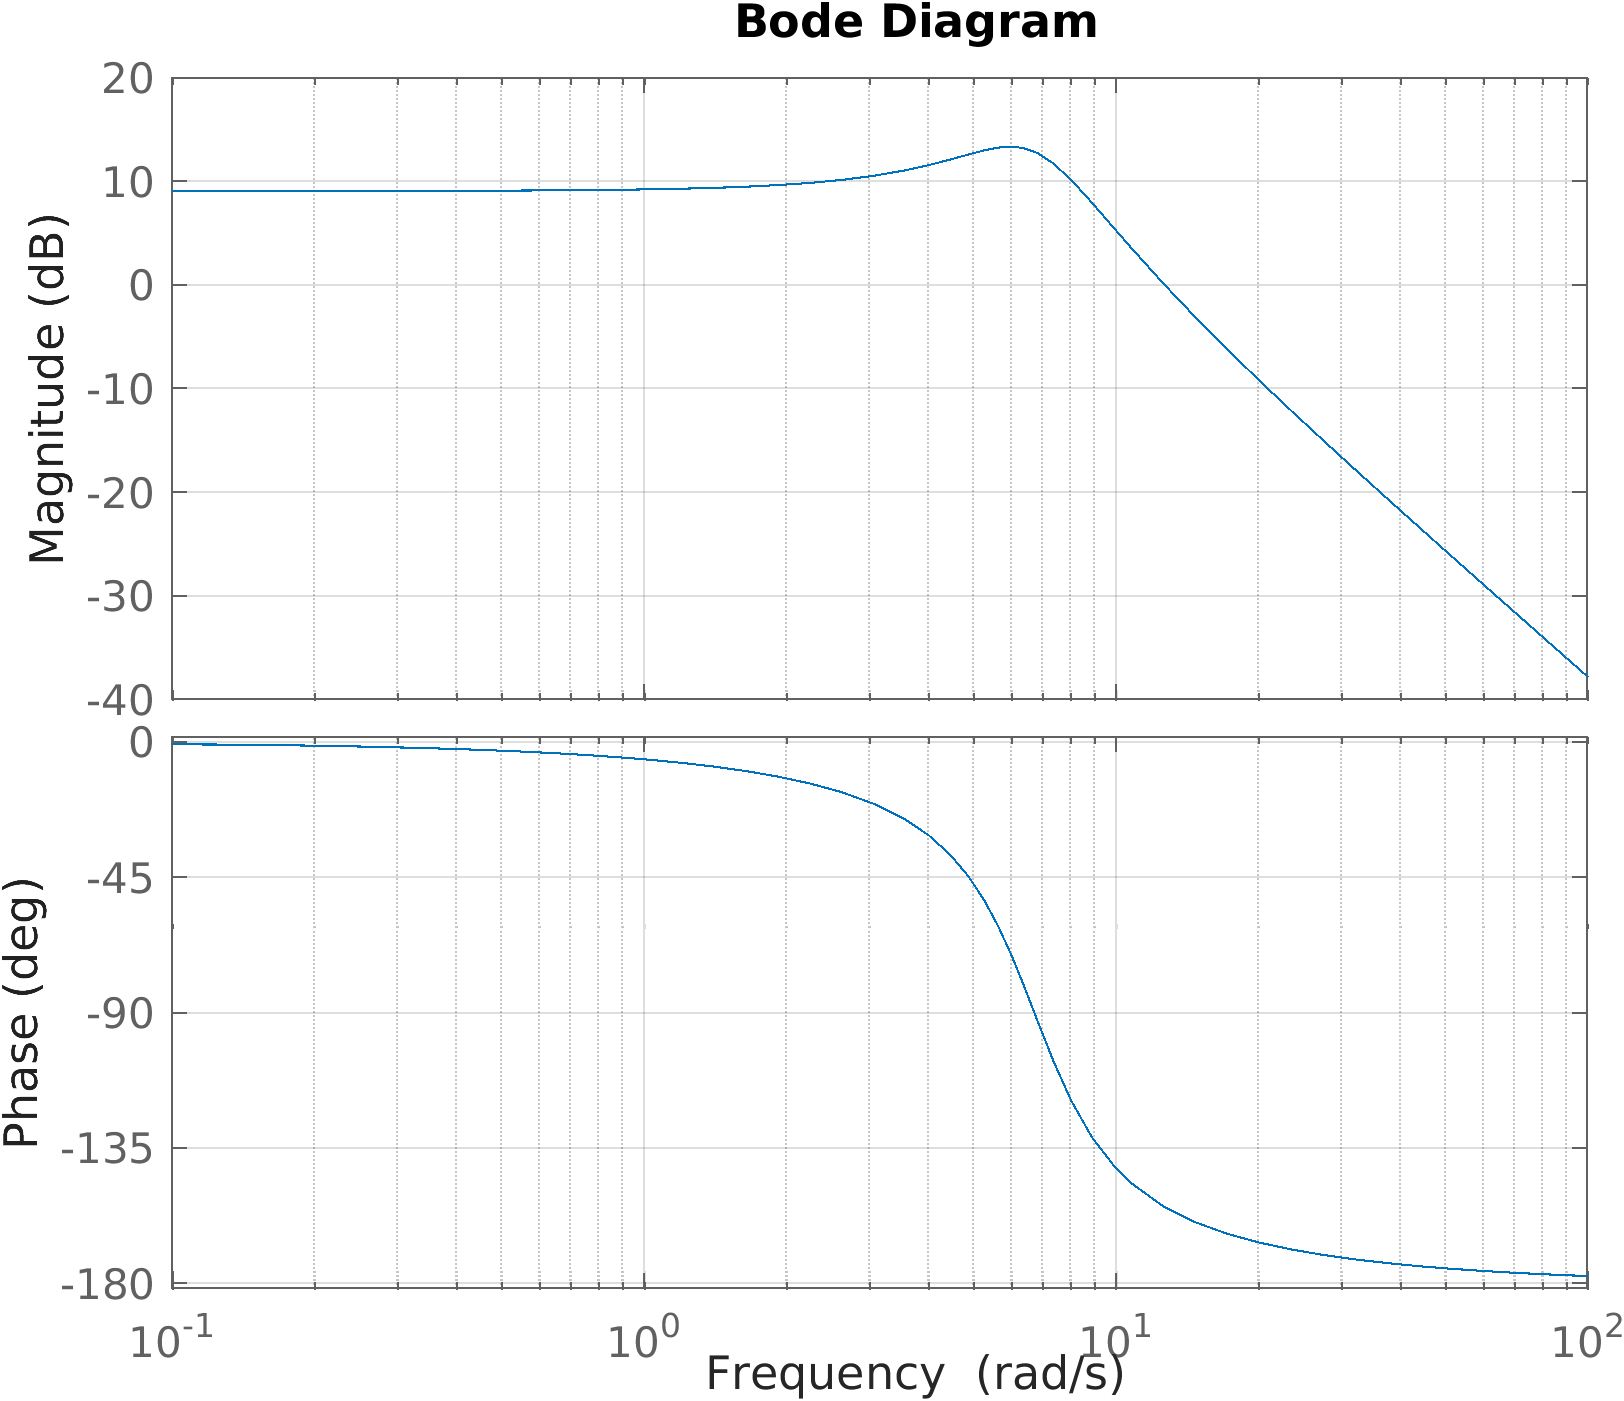
\includegraphics[width=0.7\textwidth]{figs/task_2_ЛАФЧХ.png}
    \caption{ЛАФЧХ полной модели ДПТ.}
    \label{fig:task_2_ЛАФЧХ}
\end{figure}


\section{Конденсатор}

Дано уравнение конденсатора:
\begin{equation*}
    I=C\dot U.
\end{equation*}
Входом объекта считаем $I(t)$, а выходом $U(t)$. Согласно моему варианту $C=332\ \text{мкФ}$.


\subsection{Инженерная форма ПФ}

Имеем ПФ
\begin{equation*}
    W(s)=\frac{1}{Cs},
\end{equation*}
которая соответствуем \textbf{идеальному интегрирующему звену}:
\begin{equation*}
    W(s)=\frac{K}{s},
\end{equation*}
где $K=\frac{1}{C}\approx3012$.

\subsection{Весовая функция}

Аналогично предыдущим пунктам, найдем весовую функцию ($U_{i.r.}(t)$).
\begin{equation*}
    U_{i.r.}(t)=K.
\end{equation*}
График этого решения и симуляцию можно посмотреть на рисунке \ref{fig:task_3_impl_step}.

\subsection{Переходная функция}

Аналогично предыдущим пунктам, находим переходную функцию ($U_{s.r.}(t)$).

\begin{equation*}
        \frac{W(s)}{s}=\frac{K}{s^2},\quad\rightarrow\quad
        U_{s.r.}(t)=Kt.
\end{equation*}
График этого решения и симуляцию можно посмотреть на рисунке \ref{fig:task_3_impl_step}.

\begin{figure}[htbp]
    \centering
    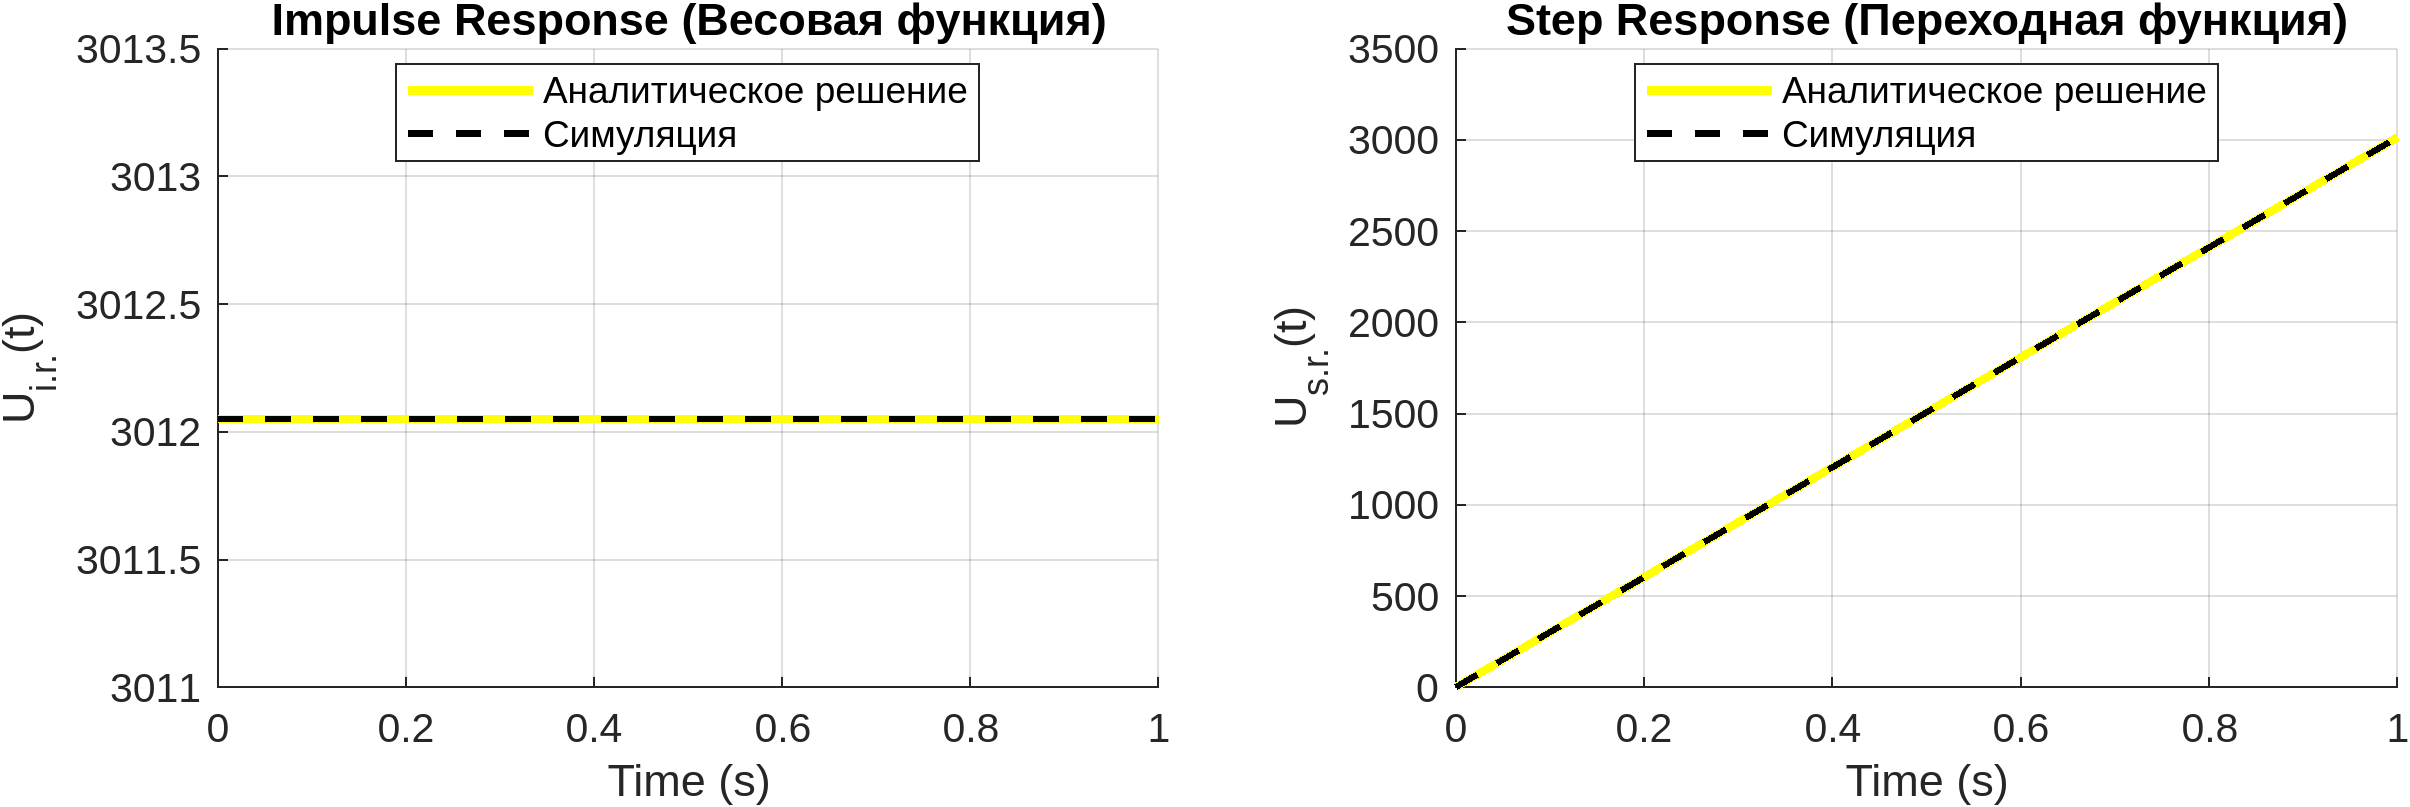
\includegraphics[width=1\textwidth]{figs/task_3_impl_step.png}
    \caption{Весовая и переходная функции уравнения конденсатора.}
    \label{fig:task_3_impl_step}
\end{figure}

\subsection{Частотные характеристики}

Найдем АФЧХ:
\begin{equation*}
    W(j\omega)=\frac{K}{j\omega}=-j\frac{K}{\omega}.
\end{equation*}
Тогда
\begin{equation*}
    A(\omega)=\sqrt{\left| \frac{K}{\omega}  \right|^2}=\left| \frac{K}{\omega}  \right|,\quad
    \varphi(\omega)=-\frac{\pi}{2}, \quad L(\omega)=20\log_{10}K-20\log_{10}|\omega|.
\end{equation*}
График АФЧХ и ЛАФЧХ можно посмотреть на рисунках \ref{fig:task_3_АФЧХ} и \ref{fig:task_3_ЛАФЧХ}.

\begin{figure}[htbp]
    \centering
    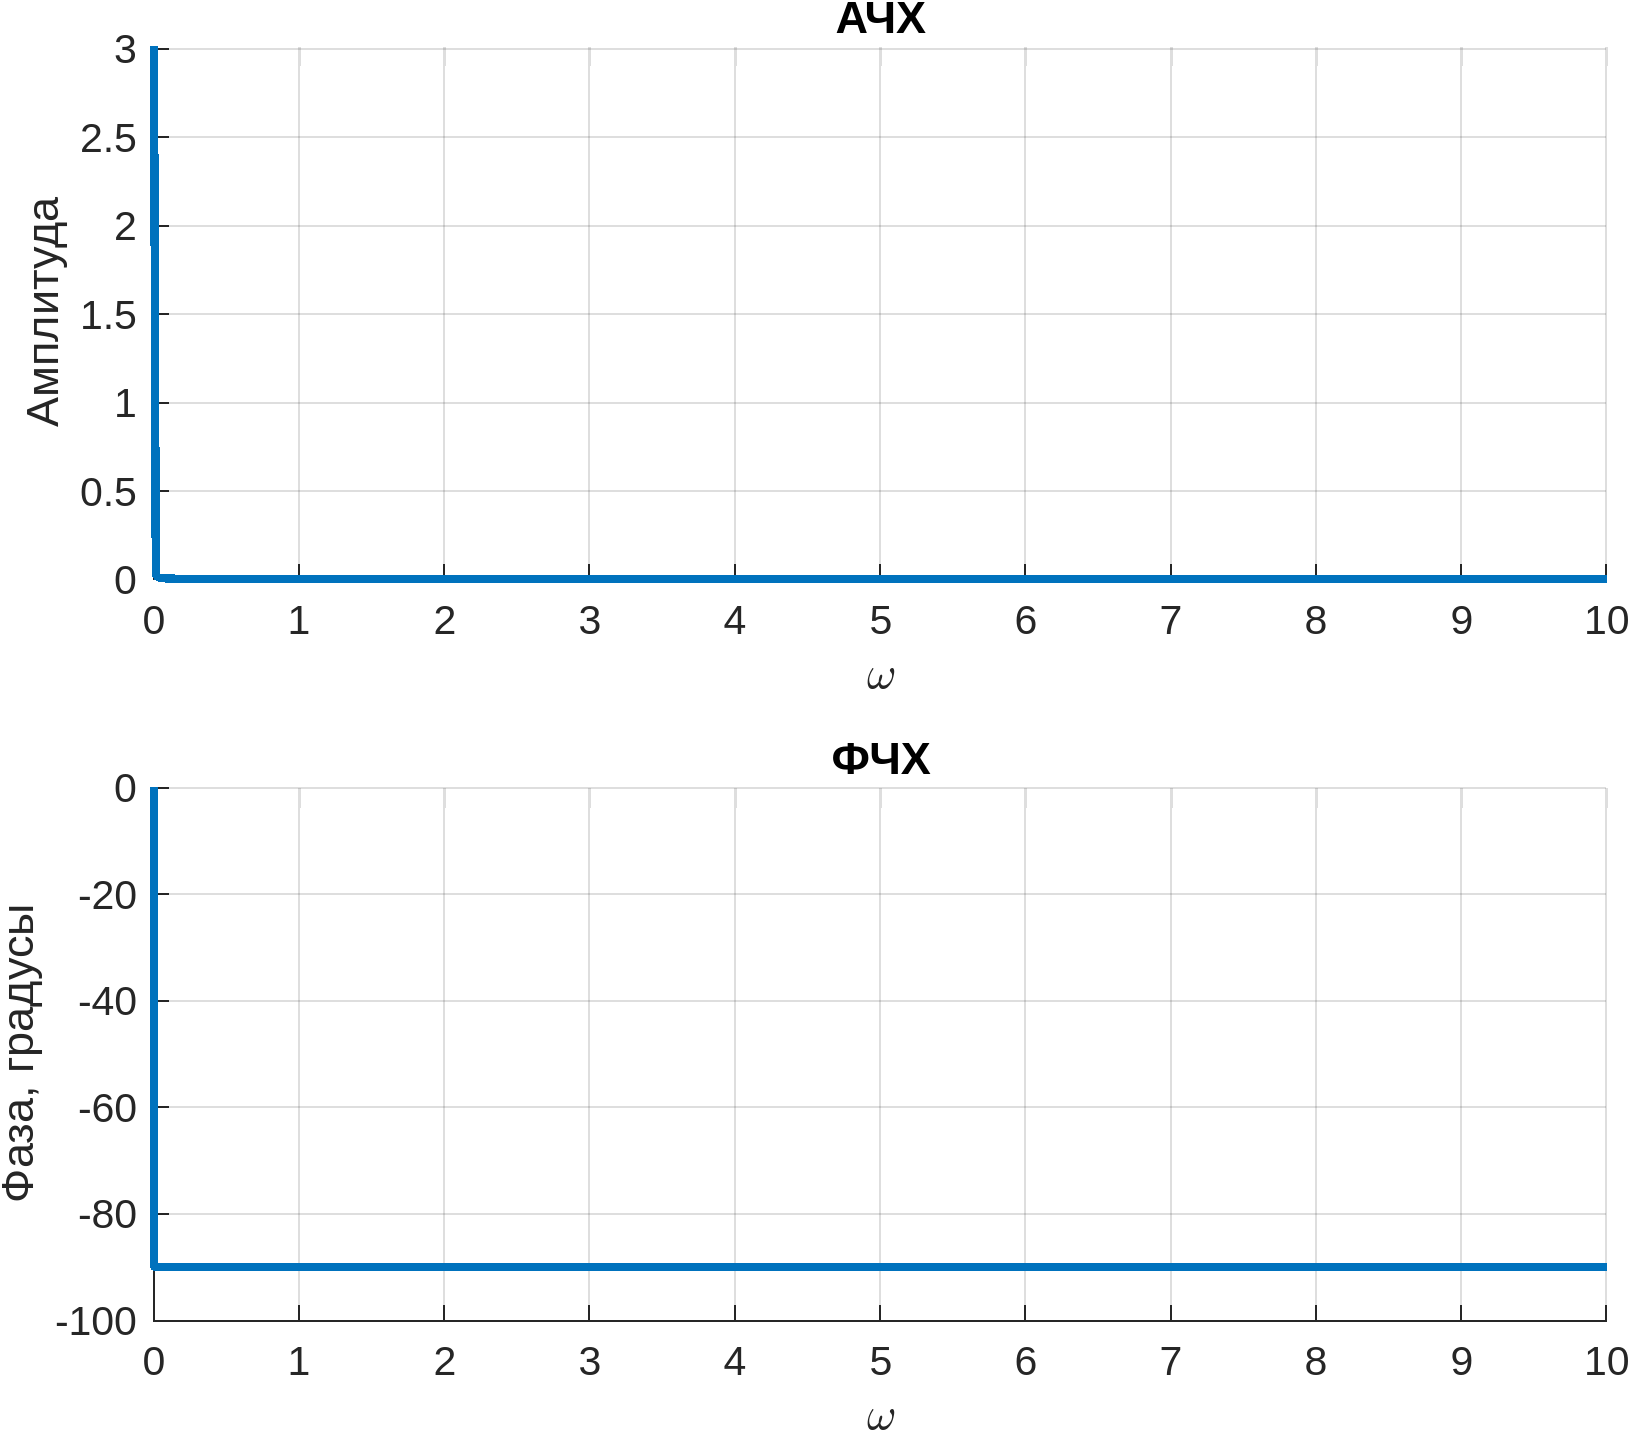
\includegraphics[width=0.7\textwidth]{figs/task_3_АФЧХ.png}
    \caption{АФЧХ уравения конденсатора.}
    \label{fig:task_3_АФЧХ}
\end{figure}

\begin{figure}[htbp]
    \centering
    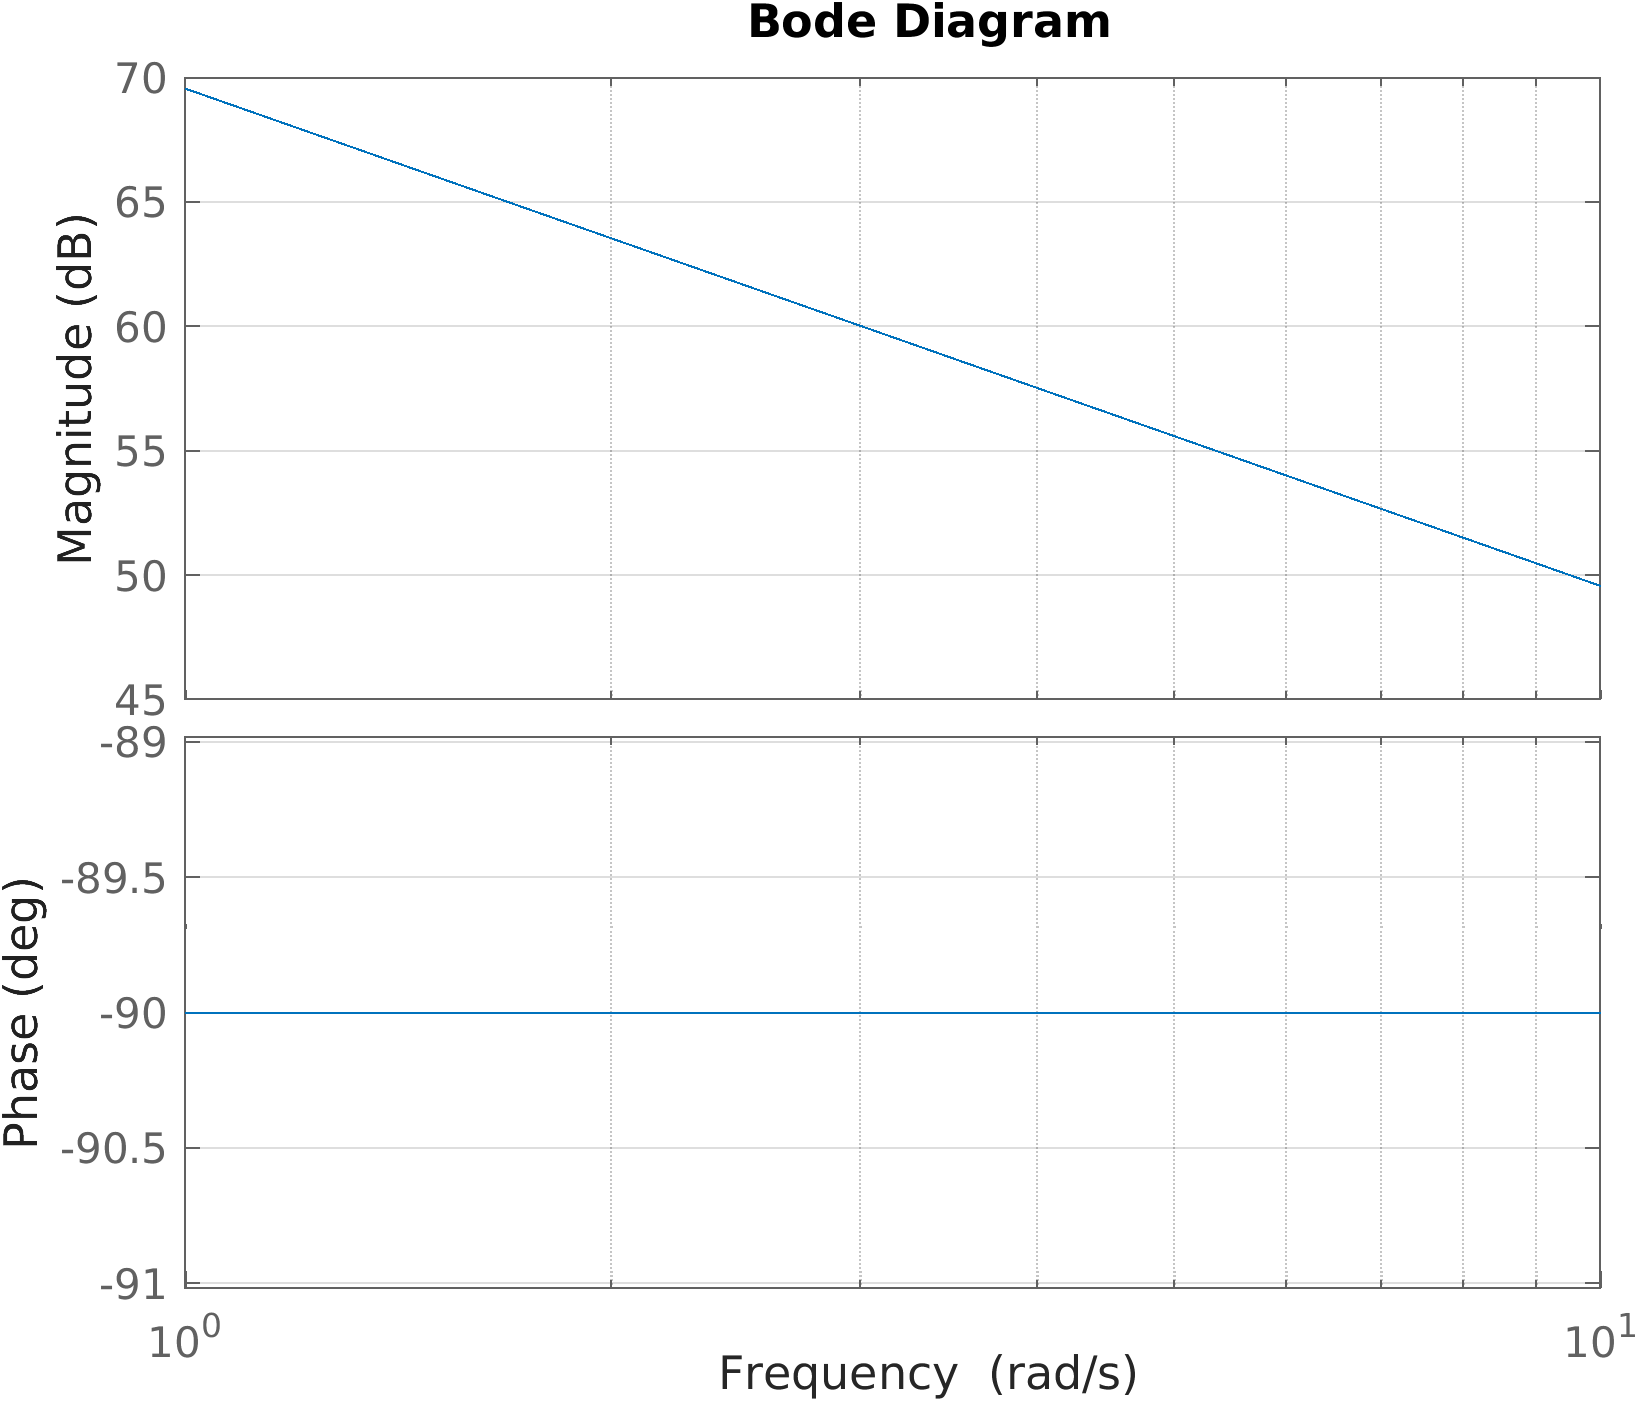
\includegraphics[width=0.7\textwidth]{figs/task_3_ЛАФЧХ.png}
    \caption{ЛАФЧХ уравения конденсатора.}
    \label{fig:task_3_ЛАФЧХ}
\end{figure}

\newpage
\section{Пружина}

\subsection{Инженерная форма ПФ}

Даны уравнения пружинного маятника:
\begin{equation*}
    F_\text{упр}=-kx,\quad F=ma.
\end{equation*}
Согласно моему варианту $k=274\ \frac{H}{m}$, $m=26\ kg$. Входом объекта 
считаем $F_{ext}(t)$ (некую внешнюю силу, направленную соосно движению маятника), 
а выходом $x(t)$. Считаем, что маятник движется ортогонально силе тяжести.
Тогда получаем диффур
\begin{equation*}
    m\ddot x+kx=F_{ext},
\end{equation*}
значит ПФ выглядит так
\begin{equation*}
    W(s)=\frac{1}{ms^2+k},
\end{equation*}
что похоже на \textbf{консервативное звено}:
\begin{equation*}
    W(s)=\frac{K}{T^2s^2+1},
\end{equation*}
где $K=\frac{1}{k}\approx 3.6 \frac{mm}{H}$, $T^2=\frac{m}{k}$, $T\approx 0.3\ \frac{kg\cdot H}{m}$

\subsection{Весовая функция}

Аналогично предыдущим пунктам, найдем весовую функцию ($x_{i.r.}(t)$).
\begin{equation*}
    W(s)=\frac{K}{T^2s^2+1}=\frac{K}{T}\frac{\frac{1}{T}}{s^2+\frac{1}{T^2}},
\end{equation*}
\begin{equation*}
    x_{i.r.}(t)=\frac{K}{T}\sin \frac{t}{T}.
\end{equation*}
Графики аналитического решения и симуляции можно посмотреть на рисунке \ref{fig:task_4_impl_step}.

\subsection{Переходная функция}

Аналогично предыдущим пунктам, находим переходную функцию ($x_{s.r.}(t)$).
\begin{equation*}
    \frac{W(s)}{s}=\frac{K}{s(T^2s^2+1)}=\frac{As+B}{T^2s^2+1}+\frac{C}{s},
\end{equation*}
\begin{equation*}
    K=As^2+Bs+C(T^2s^2+1),
\end{equation*}
\begin{equation*}
    \begin{cases}
        0=A+CT^2,\\
        0=B,\\
        K=C,
    \end{cases}\rightarrow
    \begin{cases}
        A=-KT^2,\\
        B=0,\\
        C=K.
    \end{cases}
\end{equation*}
Получаем
\begin{equation*}
    W(s)=\frac{-KT^2s}{T^2s^2+1}+\frac{K}{s}
    =\frac{K}{s}-K\frac{s}{s^2+\frac{1}{T^2}},
\end{equation*}
тогда
\begin{equation*}
    x_{s.r.}(t)=K(1-\cos\frac{t}{T}).
\end{equation*}
Графики аналитического решения и симуляции можно посмотреть на рисунке \ref{fig:task_4_impl_step}.

\begin{figure}[htbp]
    \centering
    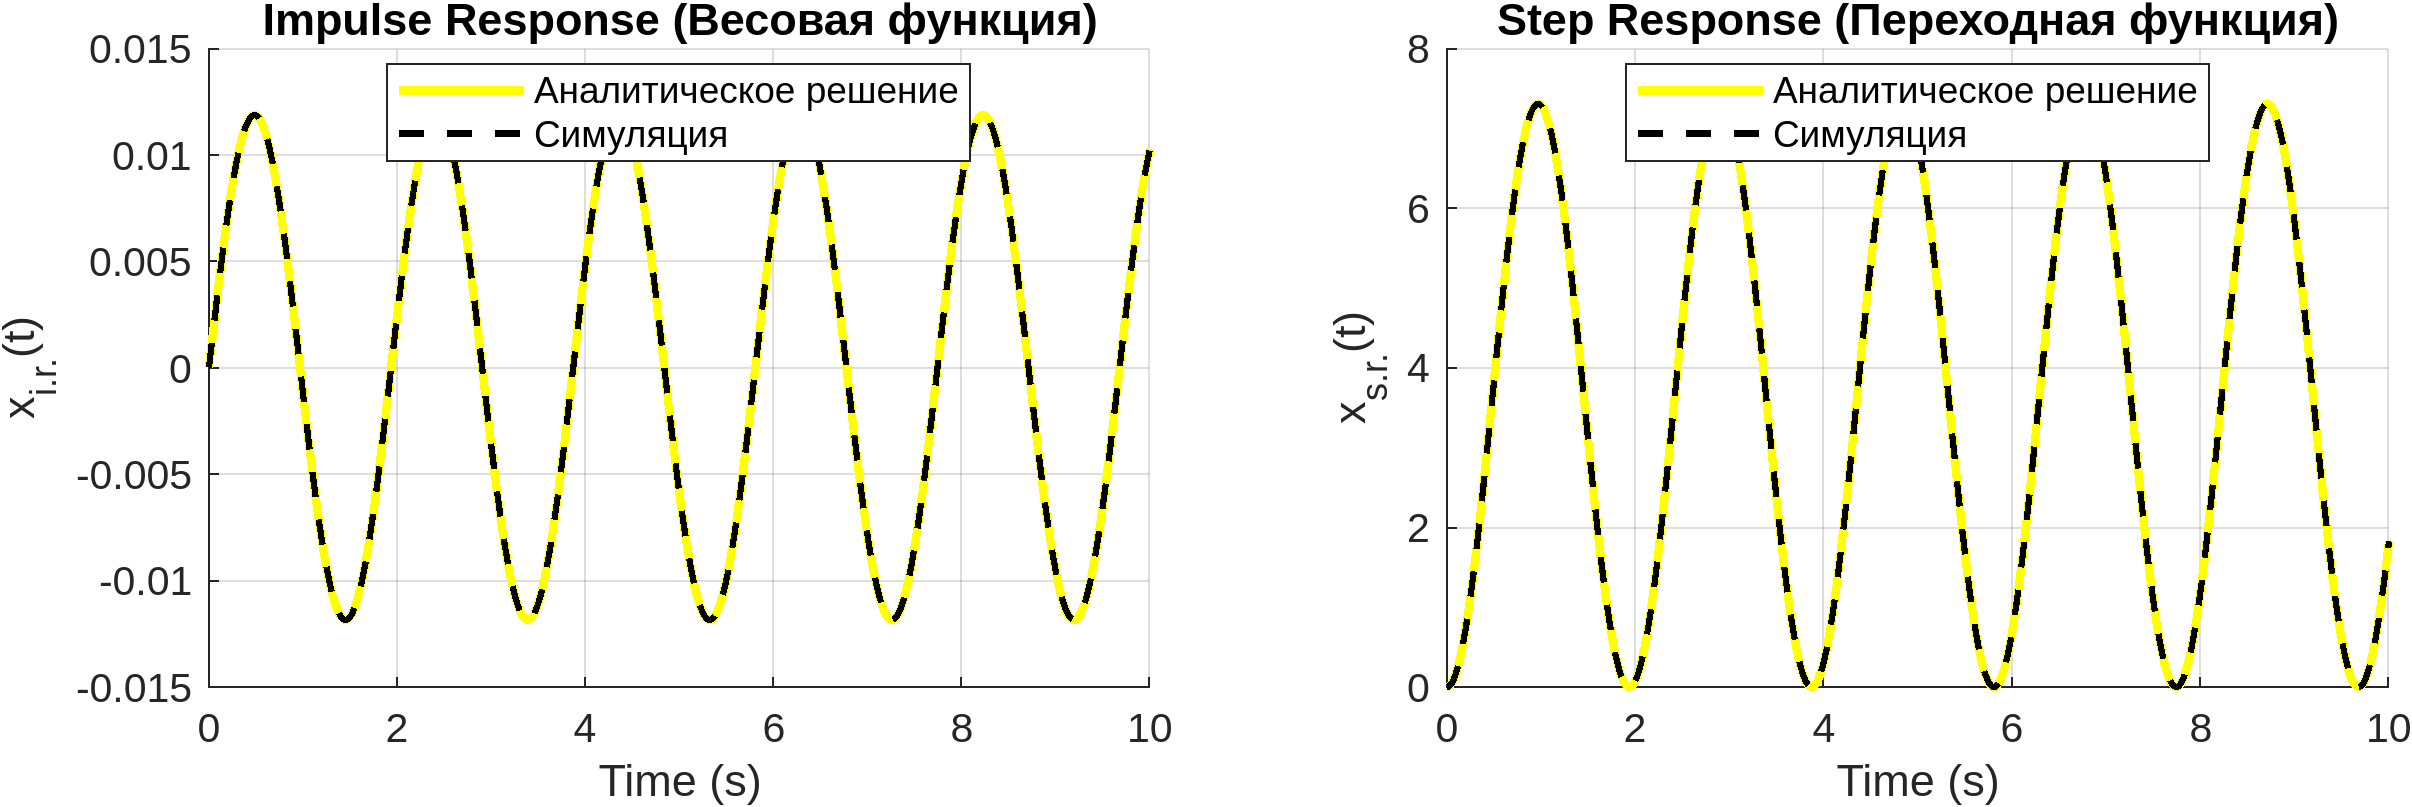
\includegraphics[width=1\textwidth]{figs/task_4_impl_step.png}
    \caption{Весовая и переходная функции пружины.}
    \label{fig:task_4_impl_step}
\end{figure}

\subsection{Частотные характеристики}

Найдем АФЧХ:
\begin{equation*}
    W(j\omega)=\frac{K}{-T^2\omega^2+1},
\end{equation*}
тогда
\begin{equation*}
    A(\omega)=\left| \frac{K}{1-T^2\omega^2} \right|, \quad L(\omega)=20\log_{10}K-20\log_{10}\left| 1-T^2\omega^2 \right|.
\end{equation*}
Так как имеем нулевую Imaginary часть, угол может быть только $\pi\cdot n,\ n\in\mathbb{Z}$, что
зависит от знака вещественной части, и так как $K$ положительно, нас интересует только $1-T^2\omega^2$ ---
это парабола с ветвями вниз и не трудно заметить, что корни $\pm\frac{1}{T}$, значит от $0$ до $\frac{1}{T}\approx 3.3$
угол равен нулю, а потом разрыв и угол становится равным $180$ или $-180$? Посмотрев на график АЧХ
(см Рис \ref{fig:task_4_АФЧХ}), мы видим, что амплитуда убывает после $3.3$, а в силу 
минимально-фазовости угол должен быть отрицателен, значит $\varphi=-180$ градусов. Значит имеем такую прерывистую функцию
фазы:
\begin{equation*}
    \varphi(\omega)=\begin{cases}
        0,& 0\leq\omega<\frac{1}{T},\\
        -\pi,& \omega>\frac{1}{T}.
    \end{cases}
\end{equation*}
Графики АФЧХ и ЛАФЧХ можно посмотреть на рисунках \ref{fig:task_4_АФЧХ} и \ref{fig:task_4_ЛАФЧХ}.

\begin{figure}[H]
    \centering
    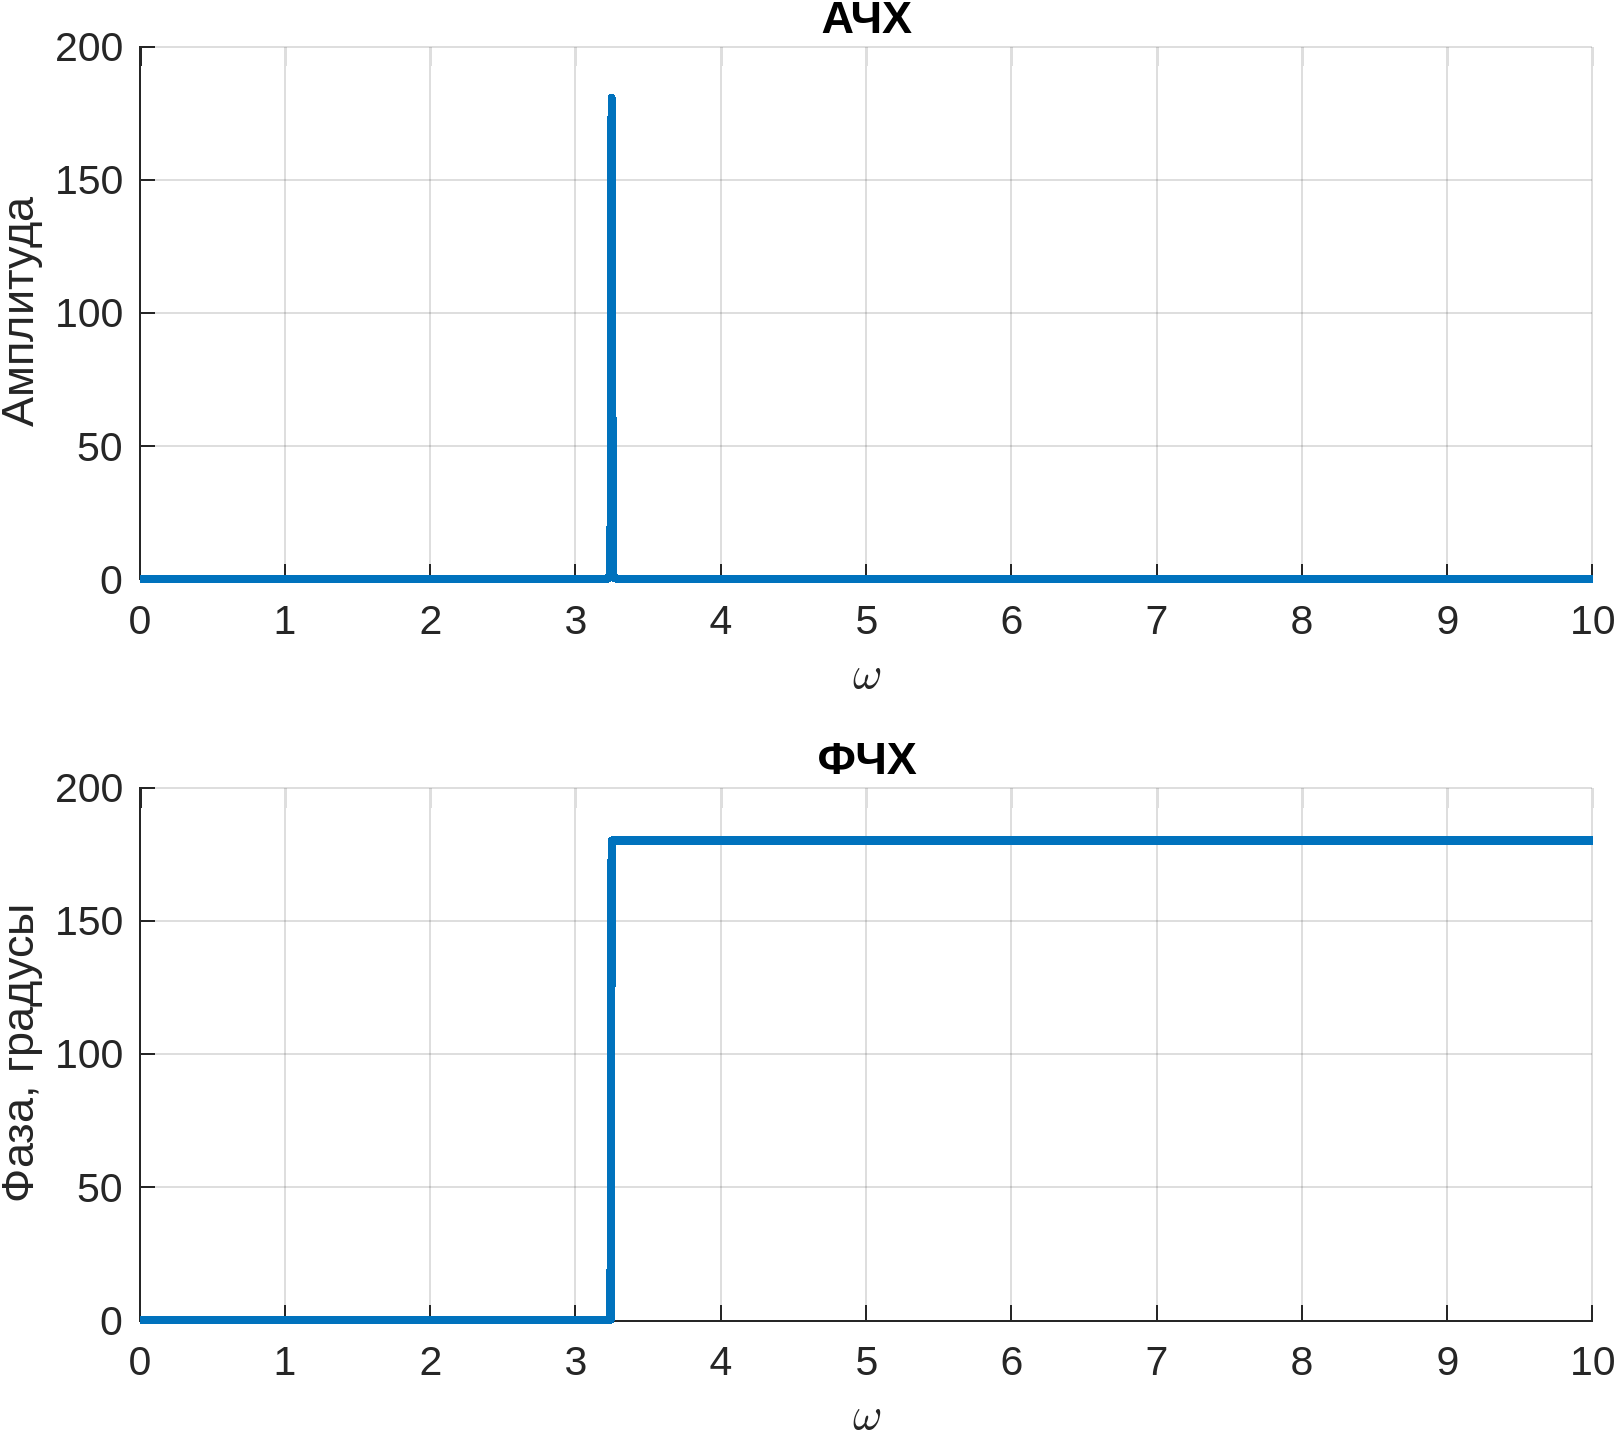
\includegraphics[width=0.7\textwidth]{figs/task_4_АФЧХ.png}
    \caption{АФЧХ пружины.}
    \label{fig:task_4_АФЧХ}
\end{figure}

\begin{figure}[H]
    \centering
    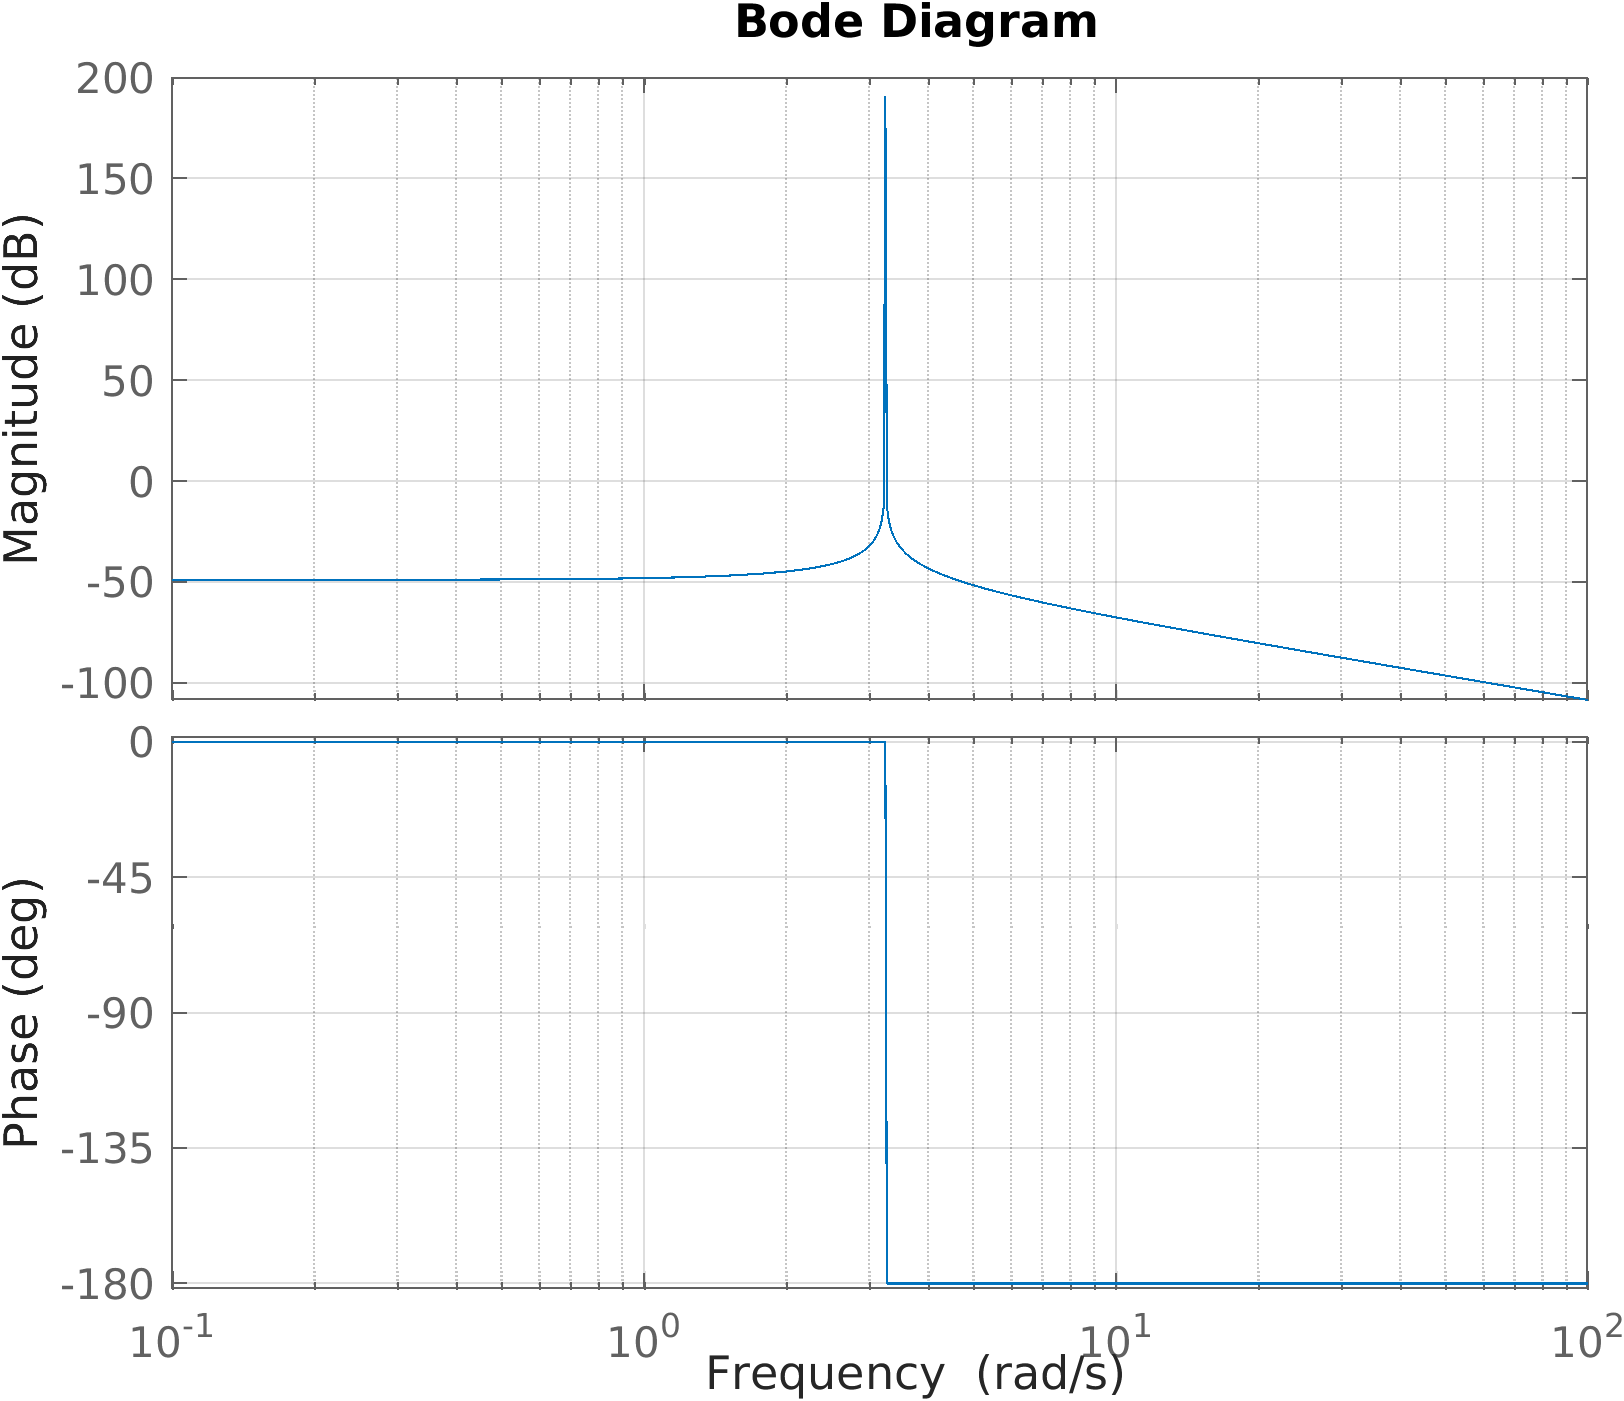
\includegraphics[width=0.7\textwidth]{figs/task_4_ЛАФЧХ.png}
    \caption{ЛАФЧХ пружины.}
    \label{fig:task_4_ЛАФЧХ}
\end{figure}


\section{ПИ регулятор на ОУ}

\subsection{Инженерная форма ПФ}

Принципиальная схема, представленная в лабораторной, является схемой ПИ регулятора на
операционном усилителе, ПФ схемы от $U_\text{ВХ}(t)$ к $U_\text{ВЫХ}(t)$
\begin{equation*}
    W(s)=\frac{R_2Cs+1}{R_1Cs},
\end{equation*}
где $R_1=3440\ \text{Ом}$, $R_2=20639\ \text{Ом}$, $C=332\ \text{мкФ}$,
согласно моему варианту. Эта ПФ соответствуем \textbf{изодромному звену}:
\begin{equation*}
    W(s)=\frac{K(Ts+1)}{s},
\end{equation*}
где $K=\frac{1}{R_1C}\approx0.87\ \frac{1}{\text{Ом}\cdot\text{Ф}}$,
$T=R_2C\approx6.85\ \text{Ом}\cdot\text{Ф}$.

\subsection{Переходная функция}

Аналогично как в предыдущих заданиях, получаем переходную функцию:
\begin{equation*}
    \frac{W(s)}{s}=K\left[ \frac{T}{s}+\frac{1}{s^2} \right] \quad\rightarrow\quad
    U_{s.r.}(t)=K(T+t).
\end{equation*}
Графики аналитического решения и симуляции можно посмотреть на рисунке \ref{fig:task_5_impl_step}.

\subsection{Весовая функция}

На этот раз найдем весовую функция как производную от переходной:
\begin{equation*}
    U_{i.r.}(t)=\dot U_{s.r.}(t)=K.
\end{equation*}
Графики аналитического решения и симуляции можно посмотреть на рисунке \ref{fig:task_5_impl_step}.

\begin{figure}[htbp]
    \centering
    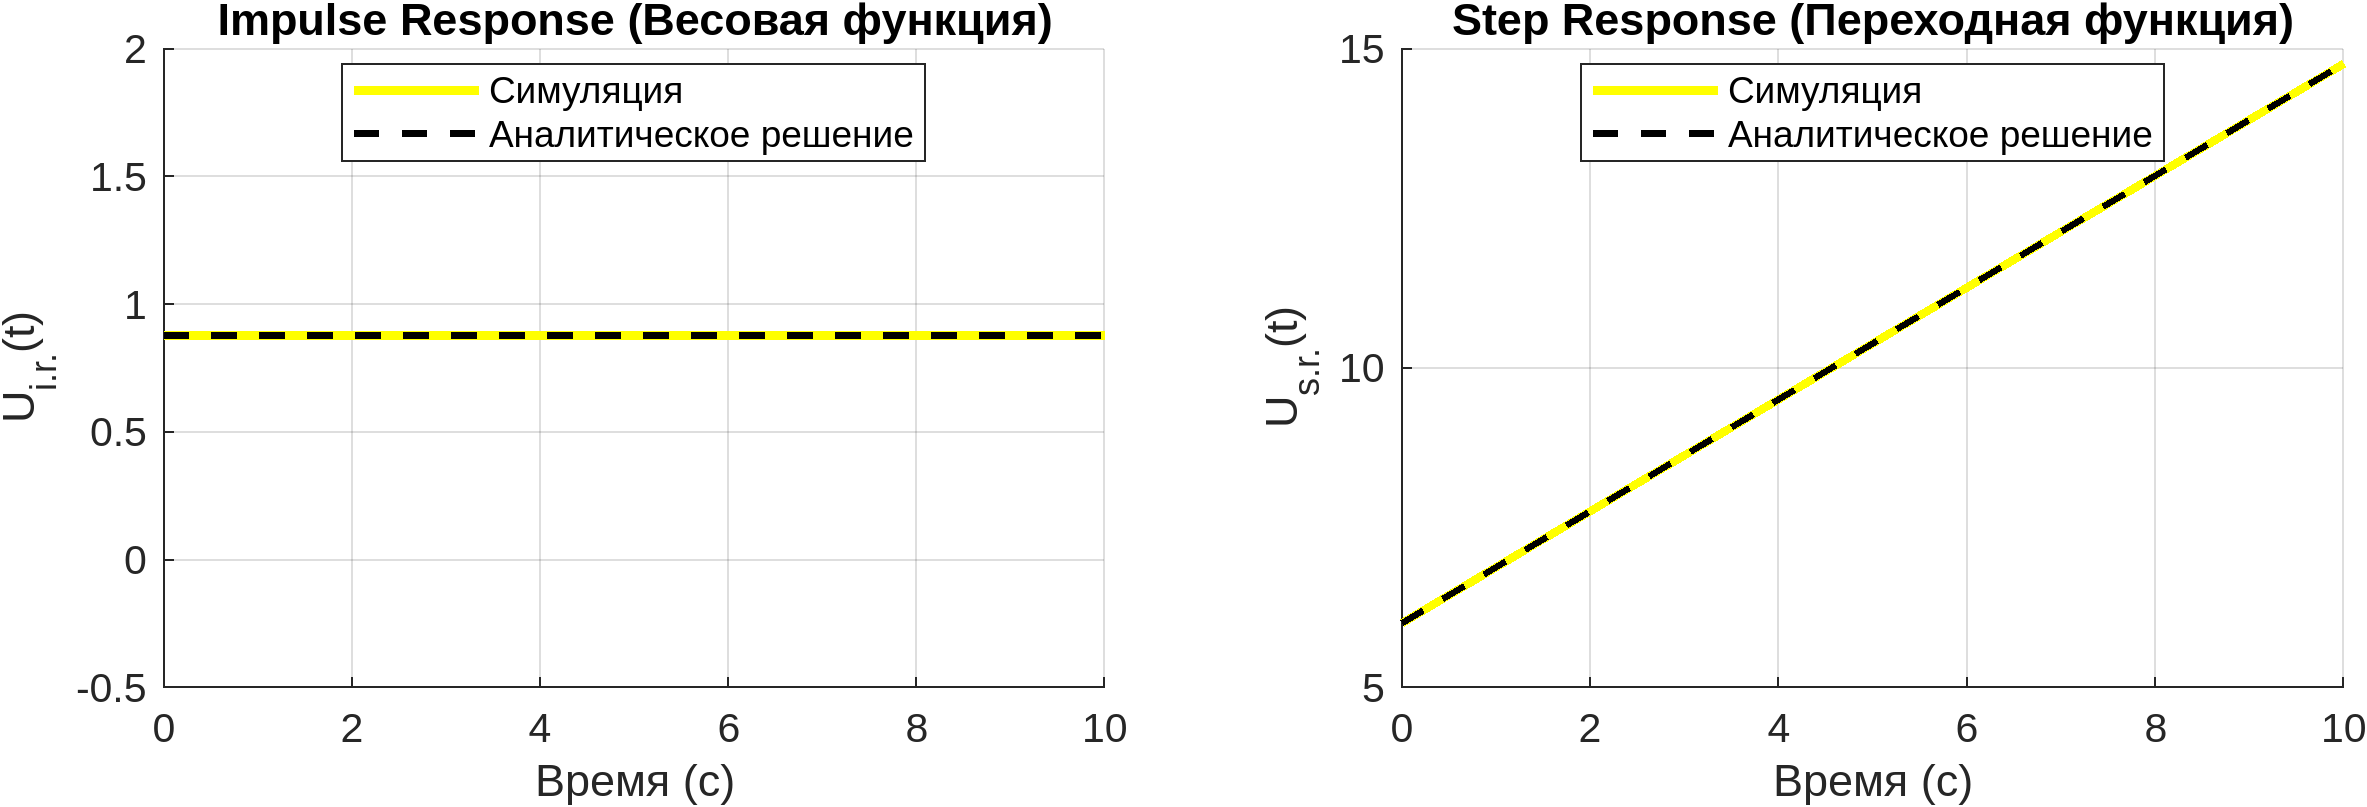
\includegraphics[width=1\textwidth]{figs/task_5_impl_step.png}
    \caption{Весовая и переходная функции ПИ регулятора на ОУ.}
    \label{fig:task_5_impl_step}
\end{figure}

\subsection{Частотные характеристики}

Найдем АЧХ и ФЧХ:
\begin{equation*}
    W(j\omega)=K\frac{Tj\omega + 1}{j\omega}=-\frac{K}{\omega}(-T\omega+j)=KT-j\frac{K}{\omega},
\end{equation*}
тогда
\begin{equation*}
    A(\omega)=K\sqrt{T^2+\frac{1}{\omega^2}},\quad \varphi(\omega)=\text{arctan}\ \frac{-1}{T\omega}, \quad L(\omega)=20\log_{10}K+10\log_{10}\left(T^2+\frac{1}{\omega^2}\right).
\end{equation*}
Графики АФЧХ и ЛАФЧХ можно посмотреть на рисунках \ref{fig:task_5_АФЧХ} и \ref{fig:task_5_ЛАФЧХ}.

\begin{figure}[H]
    \centering
    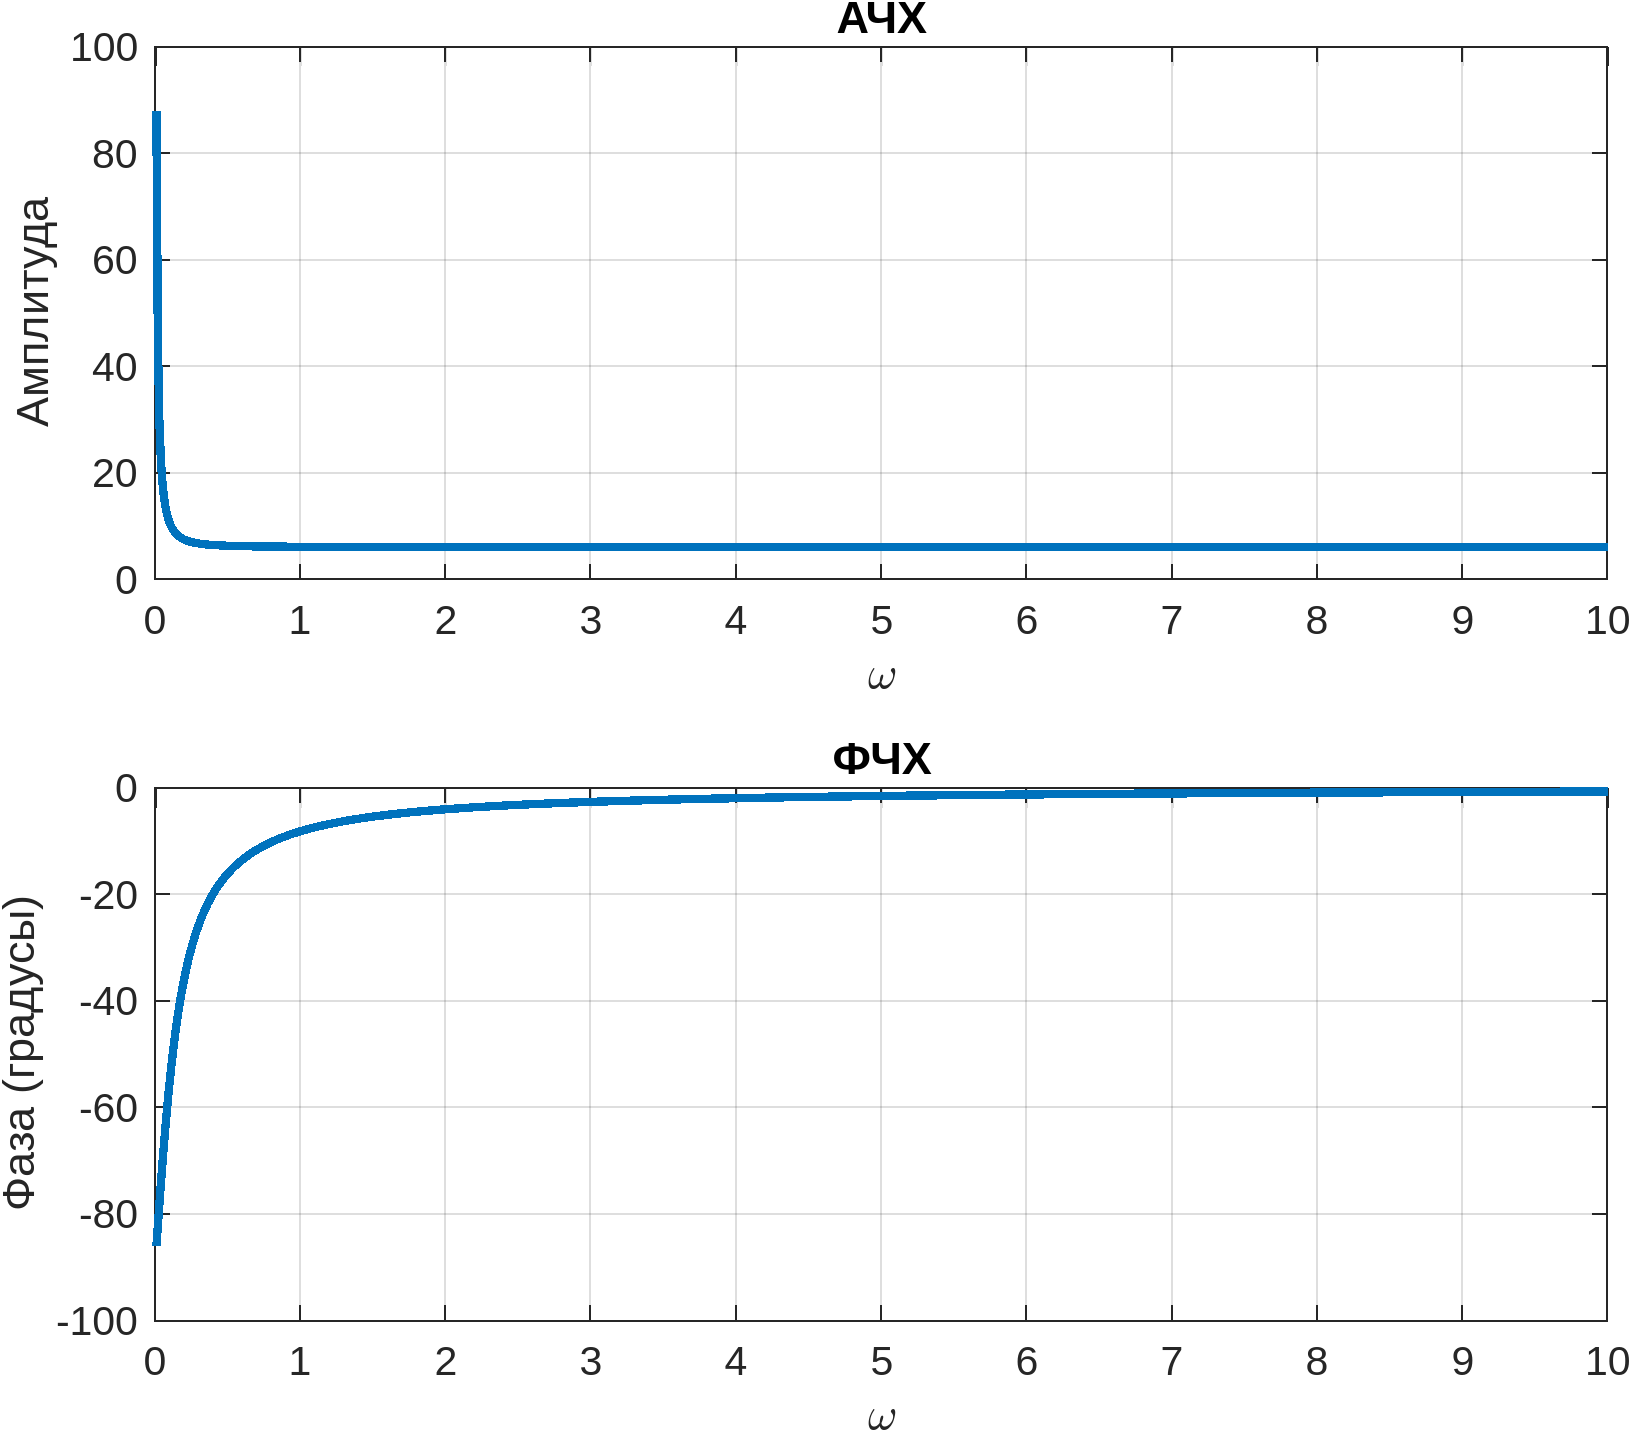
\includegraphics[width=0.7\textwidth]{figs/task_5_АФЧХ.png}
    \caption{АФЧХ ПИ регулятора на ОУ.}
    \label{fig:task_5_АФЧХ}
\end{figure}

\begin{figure}[H]
    \centering
    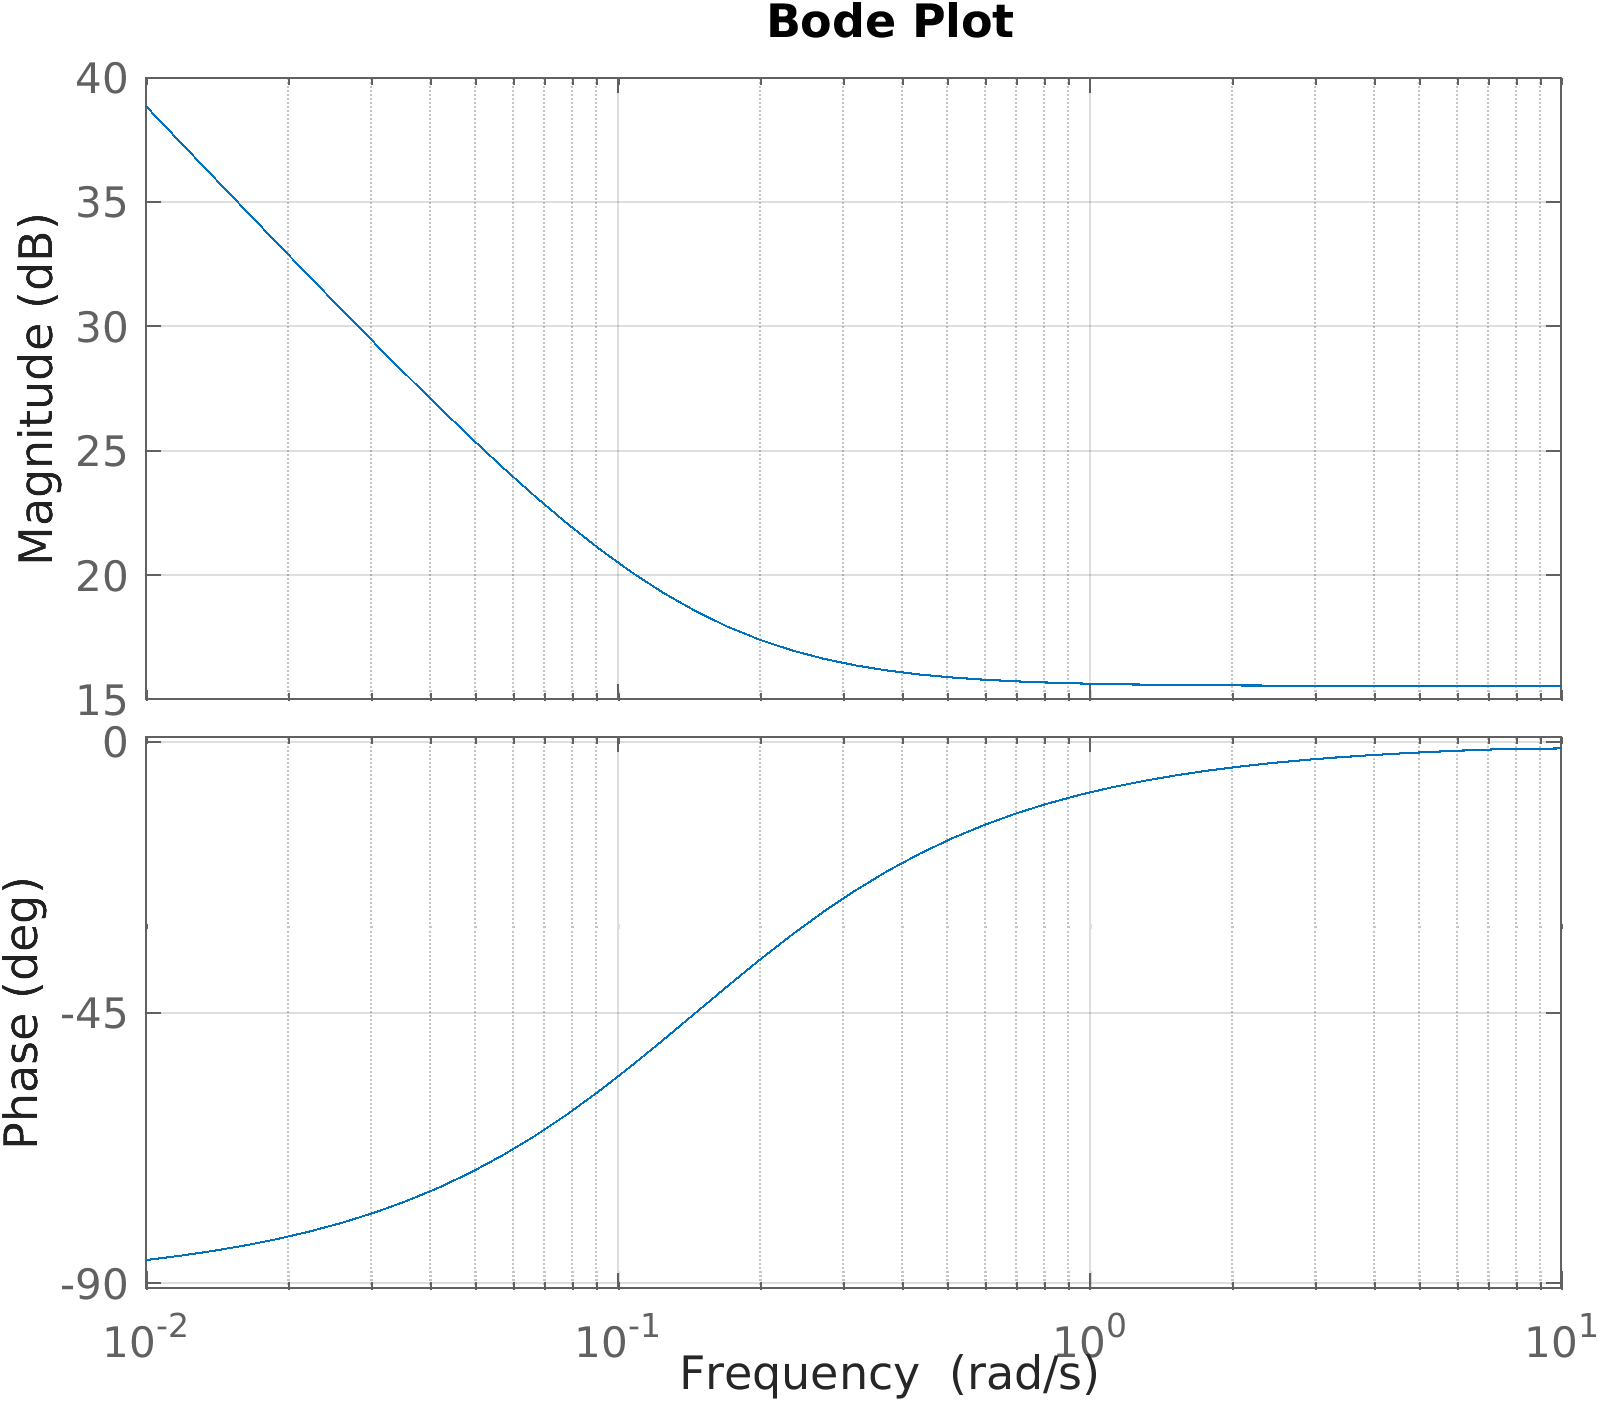
\includegraphics[width=0.7\textwidth]{figs/task_5_ЛАФЧХ.png}
    \caption{ЛАФЧХ ПИ регулятора на ОУ.}
    \label{fig:task_5_ЛАФЧХ}
\end{figure}


\section{Заключение}

В процессе выполнения этой лабораторной работы были исследованы различные
типовые звенья и их физические реализации. Для каждого примера были найдены
аналитически весовые и переходные функции, а также частотные характеристики,
которые были подтверждены симуляцией в MATLAB. Все вычисления успешно
сошлись с симуляцией.
